\documentclass{article}
\usepackage{amsmath}
\usepackage{amsthm}
\usepackage{xcolor}
\usepackage{multicol}
\usepackage{multirow}
\usepackage{graphicx}
\usepackage{enumitem}
\usepackage{amssymb}
\usepackage{listings}
\usepackage[export]{adjustbox}
\usepackage{sectsty}
\usepackage[vmargin=1in]{geometry}

% \sectionfont{\itshape}


\title{%
    % \vspace{-3.5cm}
    Assignment 1 \\
    \Large COMP5115}

\author{%
    Gabriel Racz 101181470
   }

\newcommand{\tdot}{\mathrel{{.}\,{.}}\nobreak}
\renewcommand{\i}[1]{\textit{{#1}}}
\renewcommand{\b}[1]{\textbf{{#1}}}

\begin{document}
\maketitle
\pagebreak

\section{Results vs. GeomProc}
All histograms display values filtered to the 99\textsuperscript{th} percentile to
remove outliers that would make visual analysis of the data difficult.
\subsection{Mean Curvature}
\begin{center}
\b{\i{MSE: Distance from our mean curvature method to GeomProc}}
\smallbreak
\begin{tabular}{|c|c|c|c|}
    \hline
    1-ring & 2-ring & 3-ring & 4-ring \\
    \hline
    102.328 &  110.396 & 116.401 & 119.725 \\
    \hline
\end{tabular}
\end{center}

\begin{center}
    \b{\i{Curvature Value Distributions:}}
\end{center}
\adjustbox{center}{
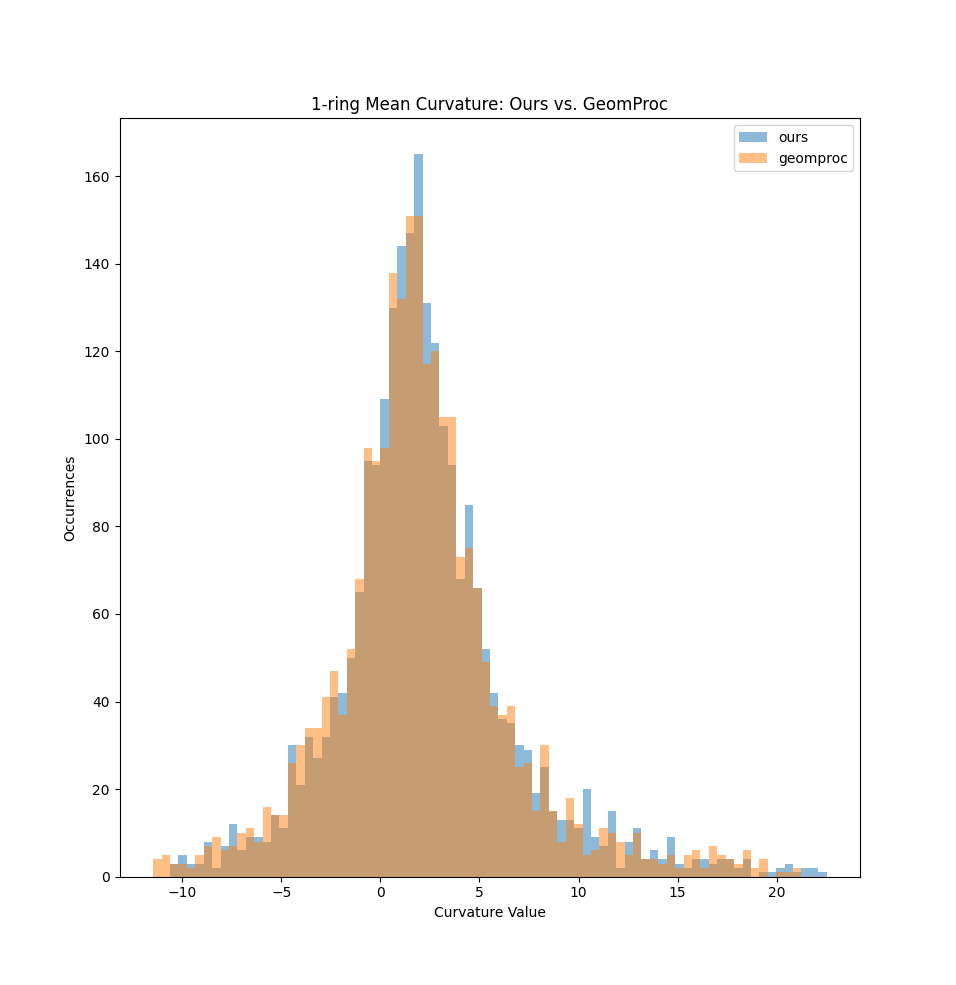
\includegraphics[width=1.5in]{mean_error_1.png}
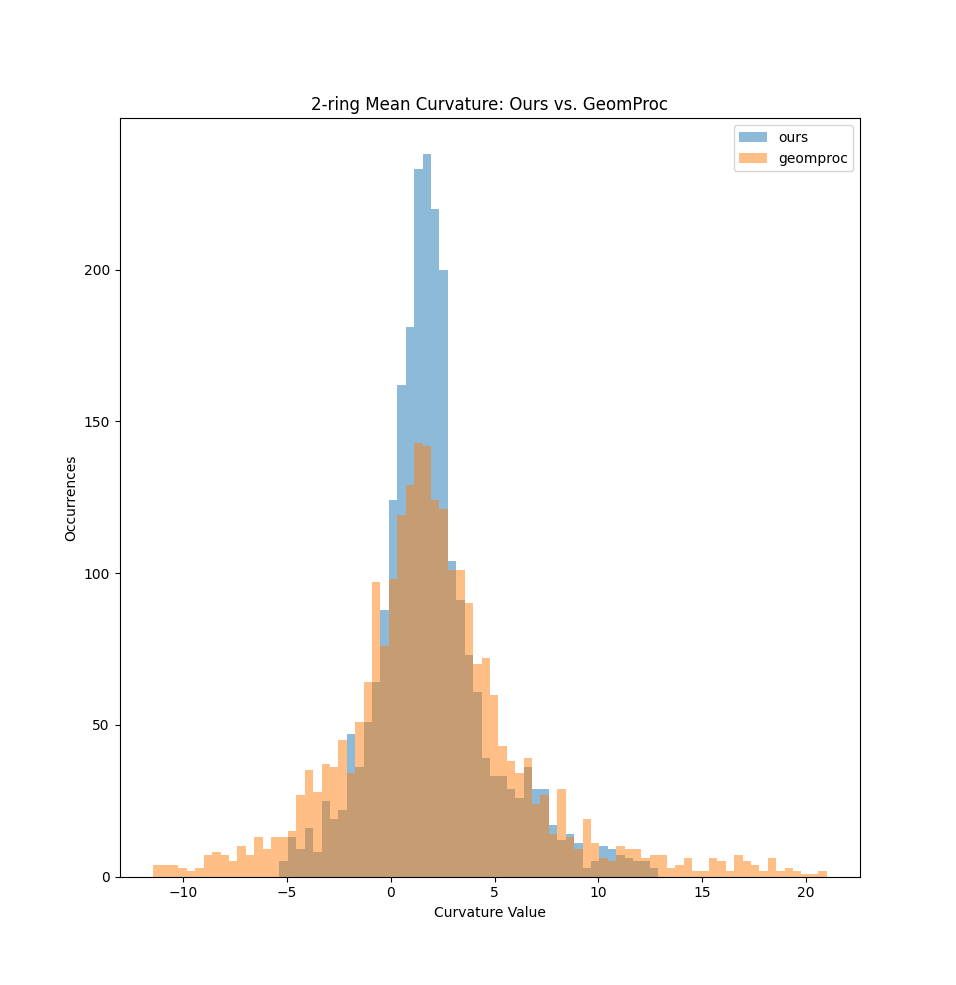
\includegraphics[width=1.4in]{mean_error_2.png}
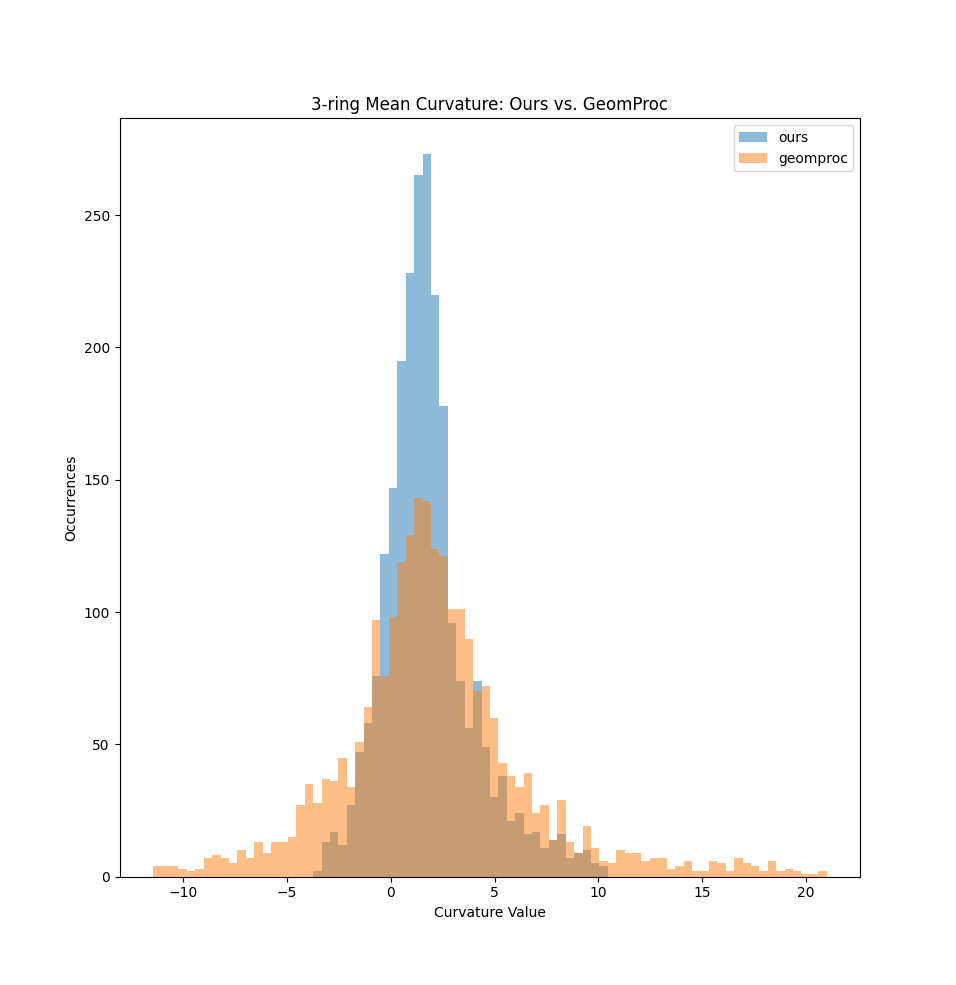
\includegraphics[width=1.5in]{mean_error_3.png}
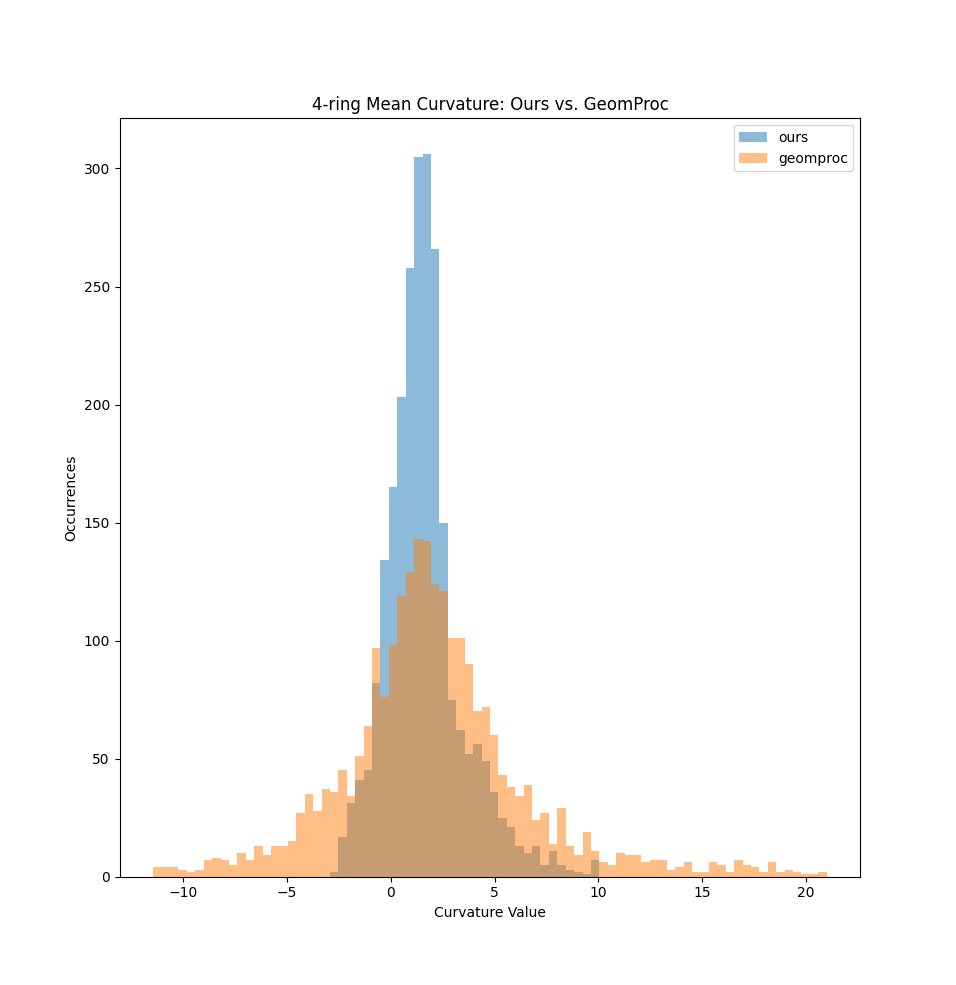
\includegraphics[width=1.5in]{mean_error_4.png}
}
\begin{center}
    \b{\i{Visual Comparison: 1 to 4-ring from left to right}}
\end{center}
\smallbreak
\adjustbox{center}{
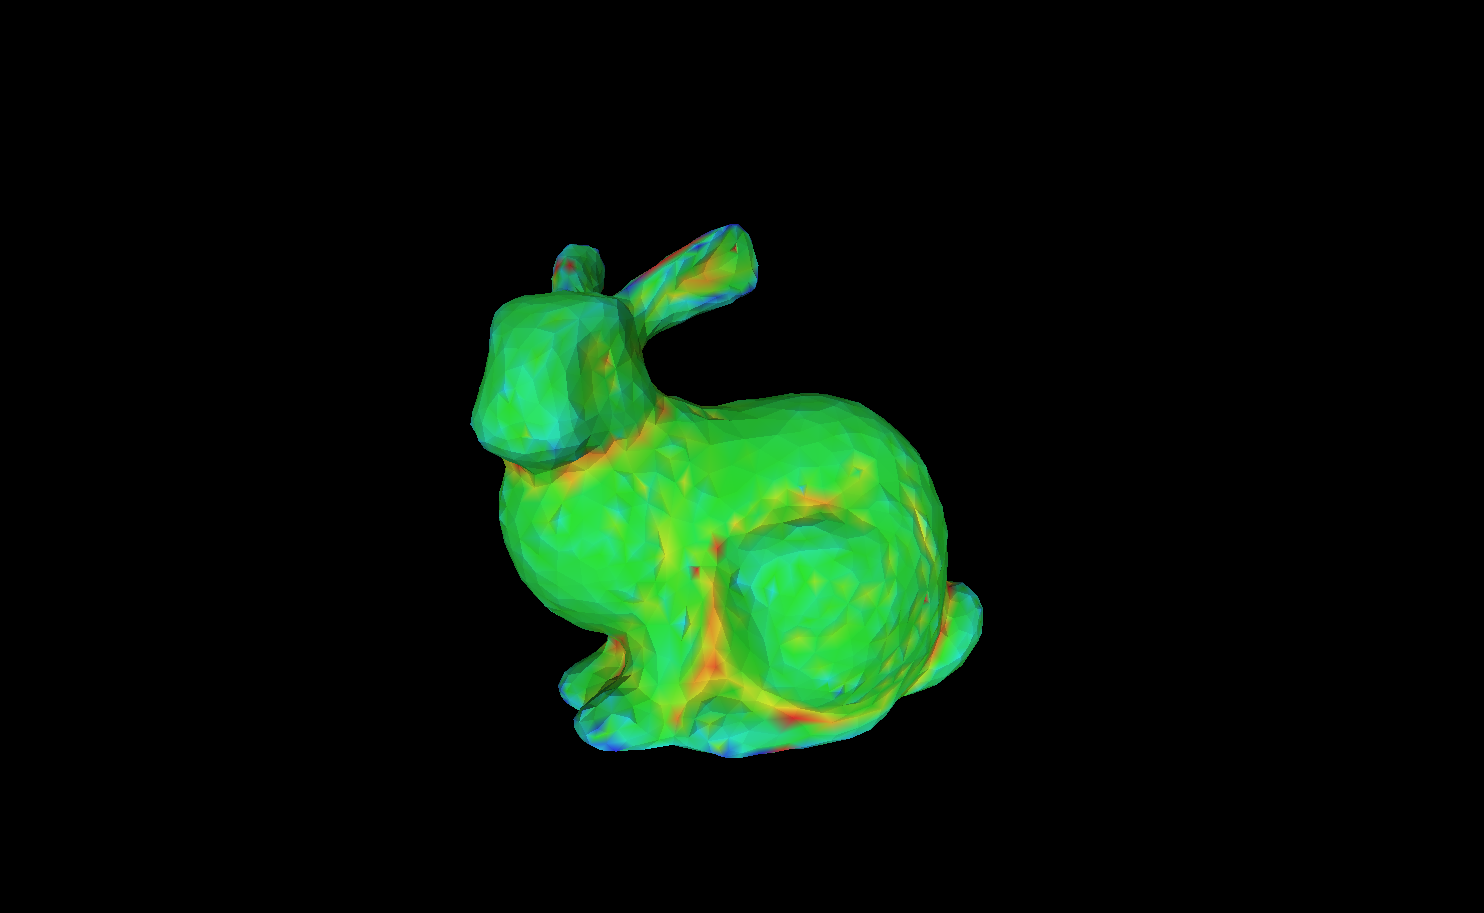
\includegraphics[width=1.5in]{mean_viz_00.png}
}
\adjustbox{center}{
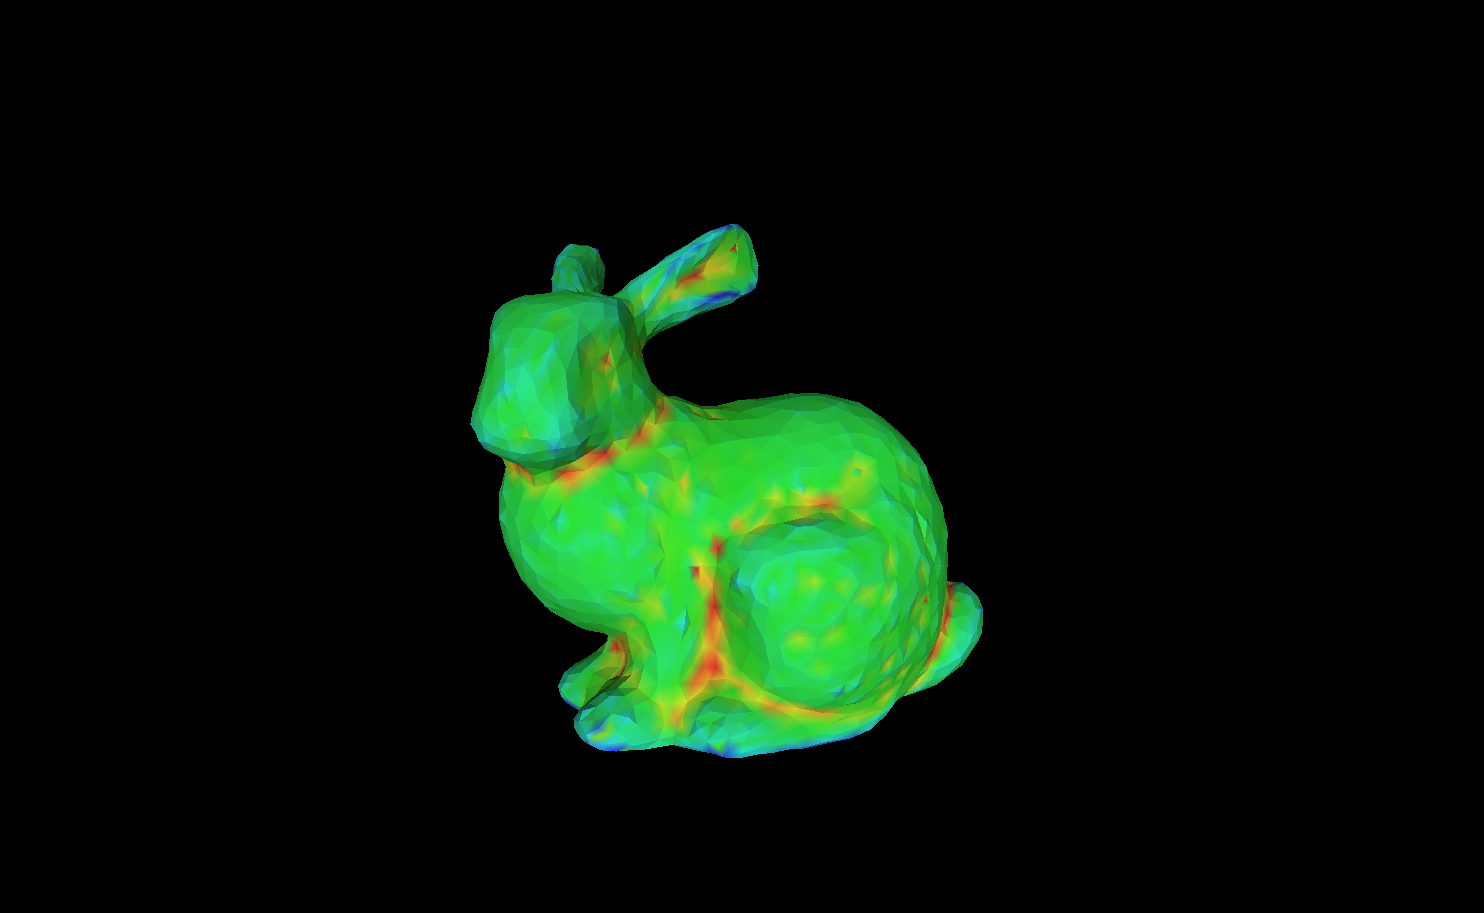
\includegraphics[width=1.5in]{mean_viz_01.png}
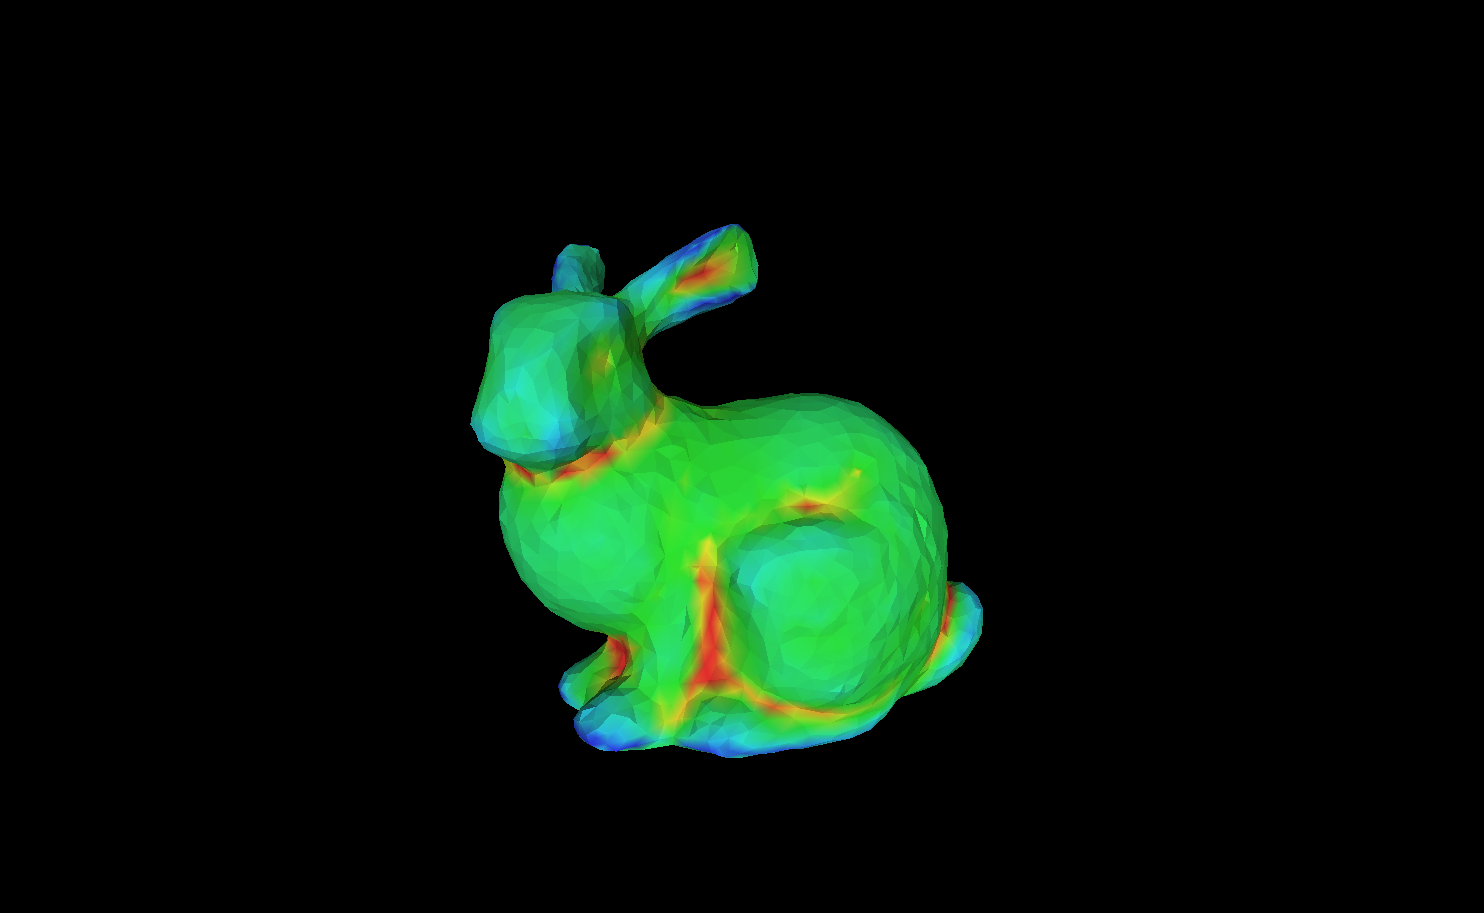
\includegraphics[width=1.5in]{mean_viz_02.png}
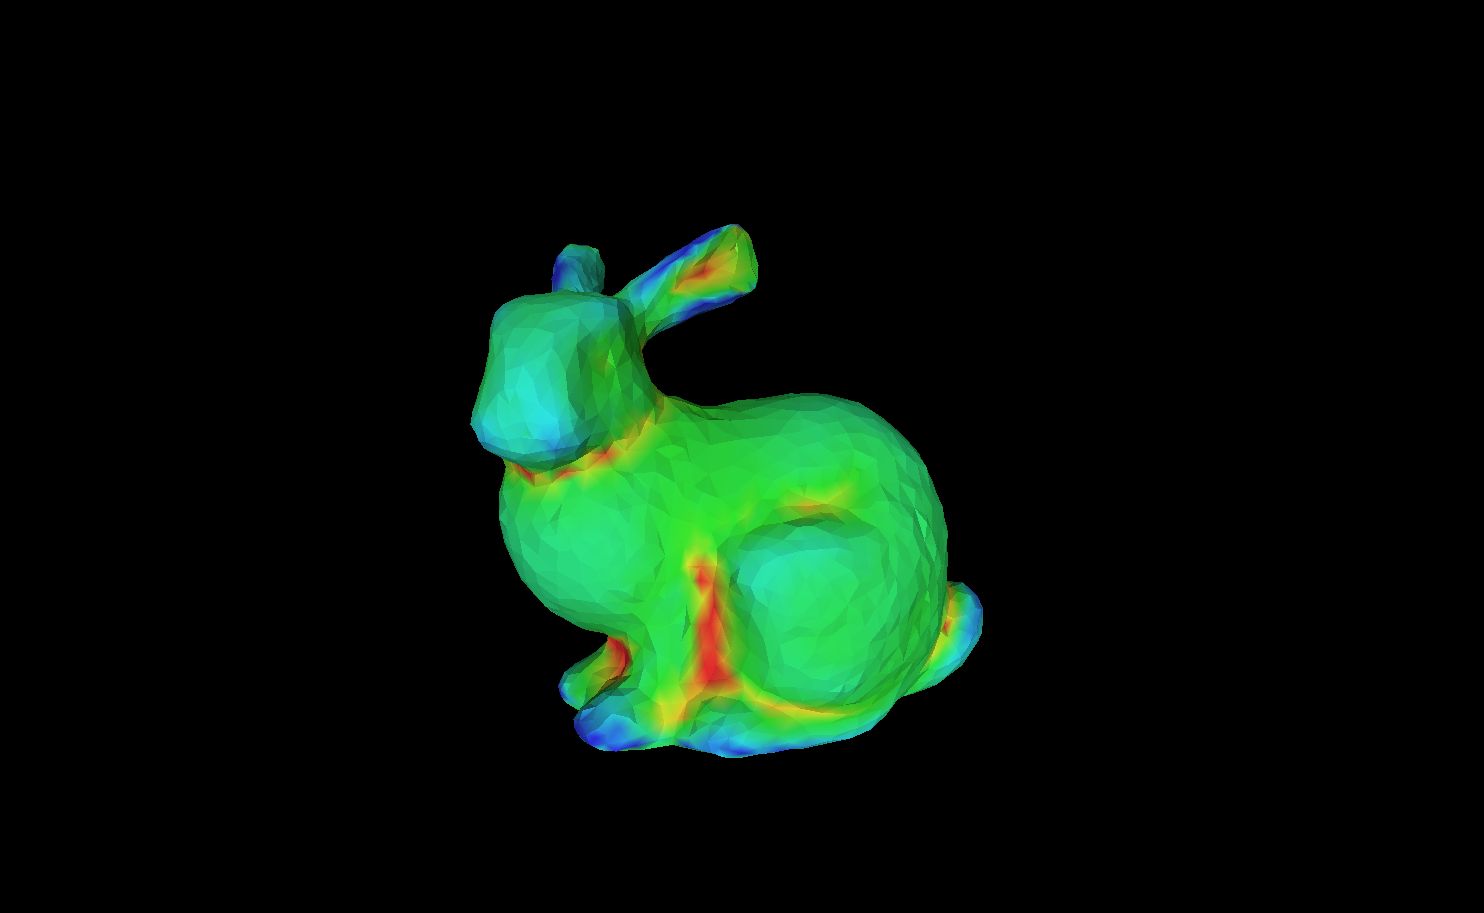
\includegraphics[width=1.5in]{mean_viz_03.png}
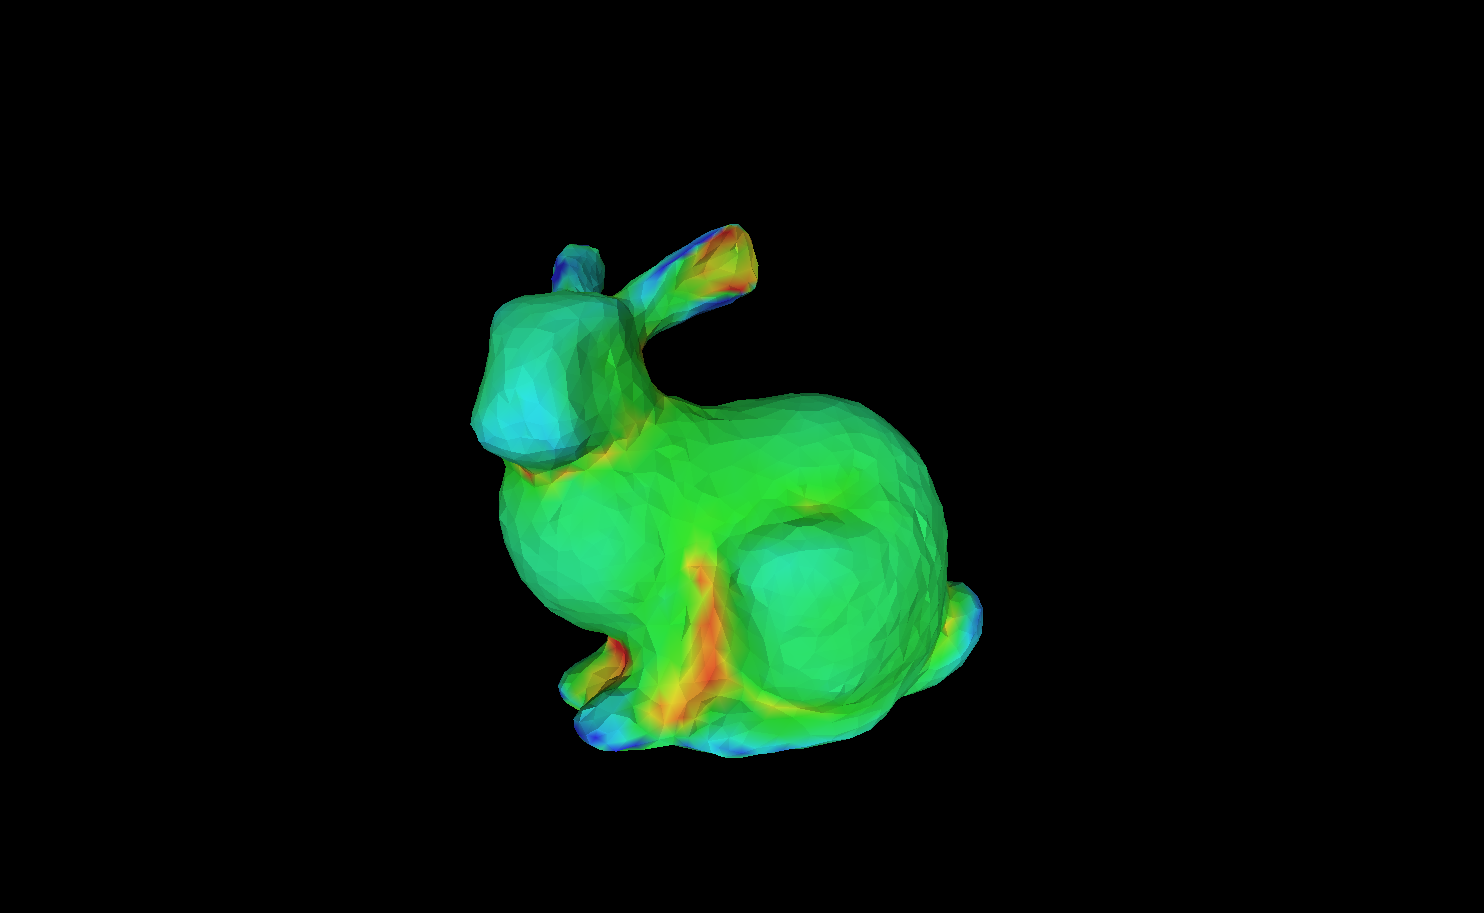
\includegraphics[width=1.5in]{mean_viz_04.png}
}

The mean curvature values computed with polynomial curve fitting match the results
produced by GeomProc quite closely. In particular, the 1-ring neighbourhood
variant has the smallest MSE. As the neighbourhood distance increases we see
the curvature values concentrate around zero due to the smoothing effect of
averaging curvature over a larger surface. The 2-ring approach of the polynomial
surface method seems to most accurately depict the topology of the mesh while
still preserving detail in small regions. When compared with the GeomProc
baseline, this approach (especially the 2-ring) does a better job at identifying
areas of convex curvature such as on the ears and feet while avoiding the
splotchy artifacts that arise from relying on only the immediate vertex
neighbours for curvature.

\pagebreak
\subsection{Gaussian Curvature}
\begin{center}
\b{\i{MSE: Distance from our gaussian curvature method to GeomProc}}
\smallbreak
\begin{tabular}{|c|c|c|c|}
    \hline
    1-ring & 2-ring & 3-ring & 4-ring \\
    \hline
    257379.800 & 244928.308 & 246108.370 & 246522.981 \\
    \hline
\end{tabular}
\end{center}
\bigbreak
\begin{center}
\b{\i{Curvature Value Distributions:}}
\end{center}
\smallbreak
\adjustbox{center}{
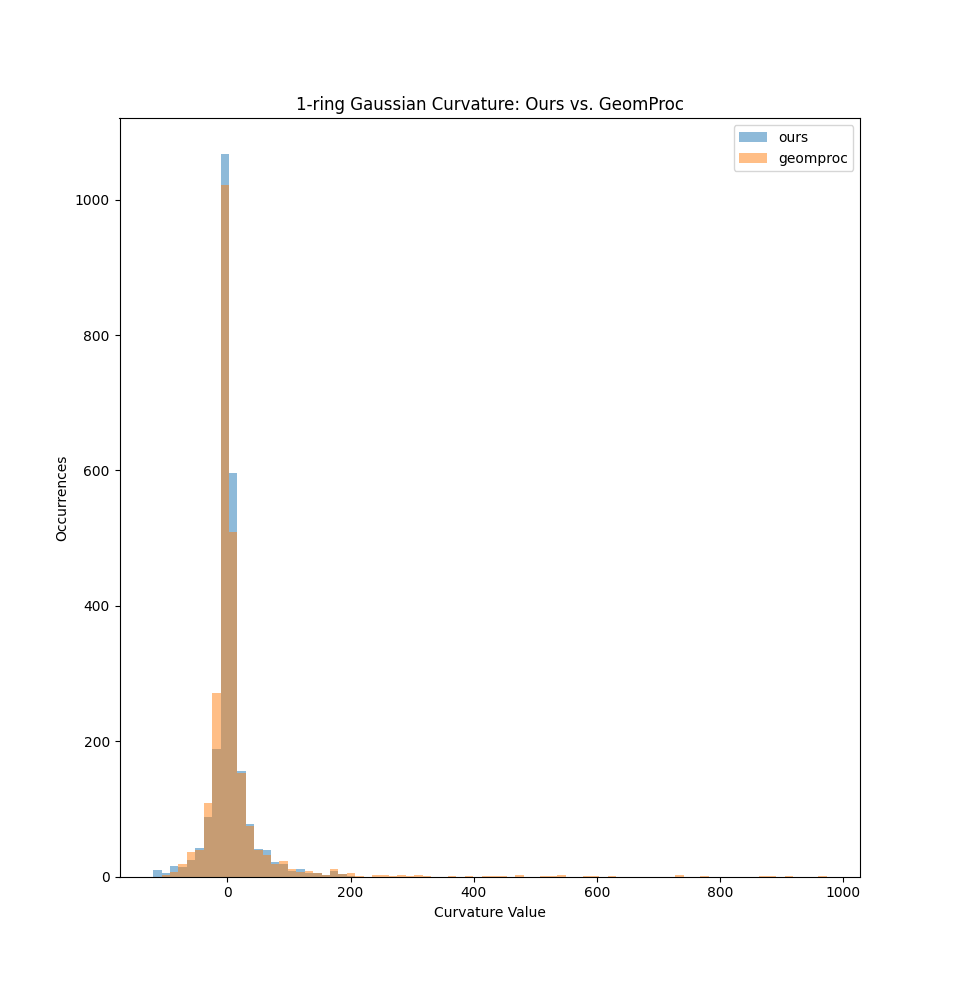
\includegraphics[width=1.5in]{gaussian_error_1.png}
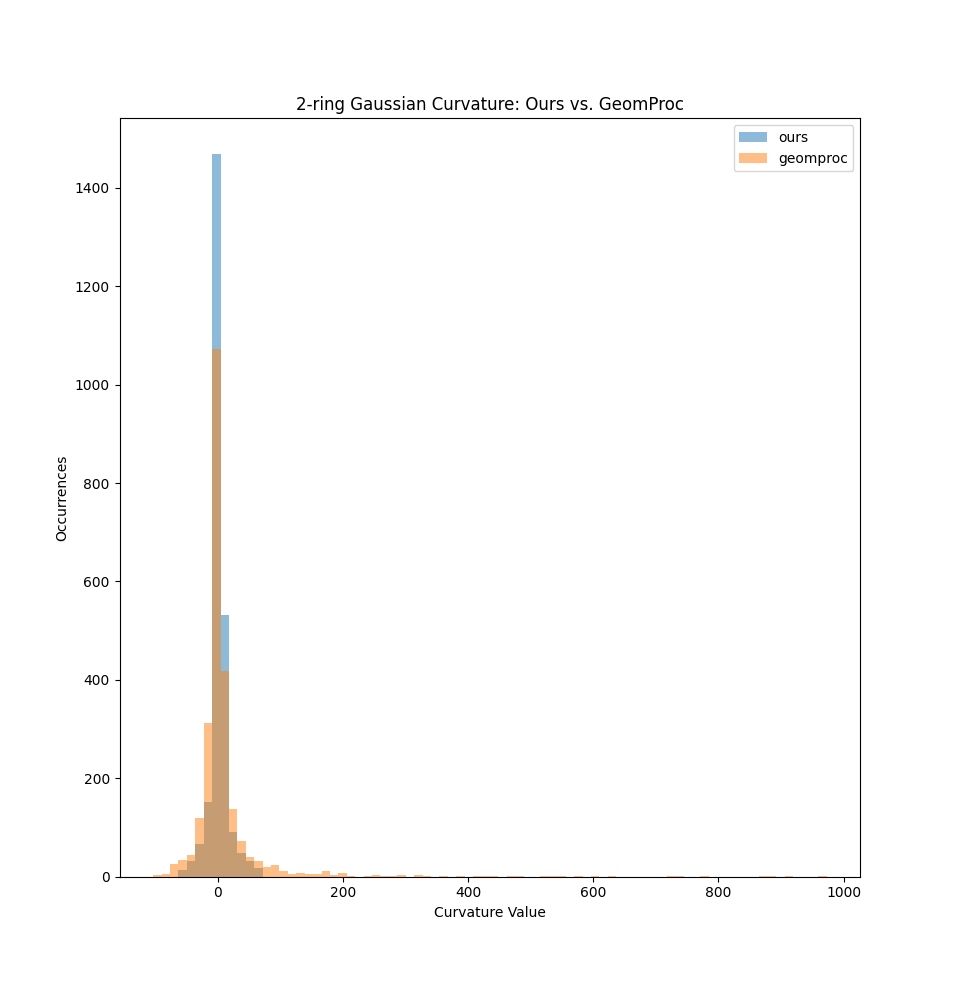
\includegraphics[width=1.5in]{gaussian_error_2.png}
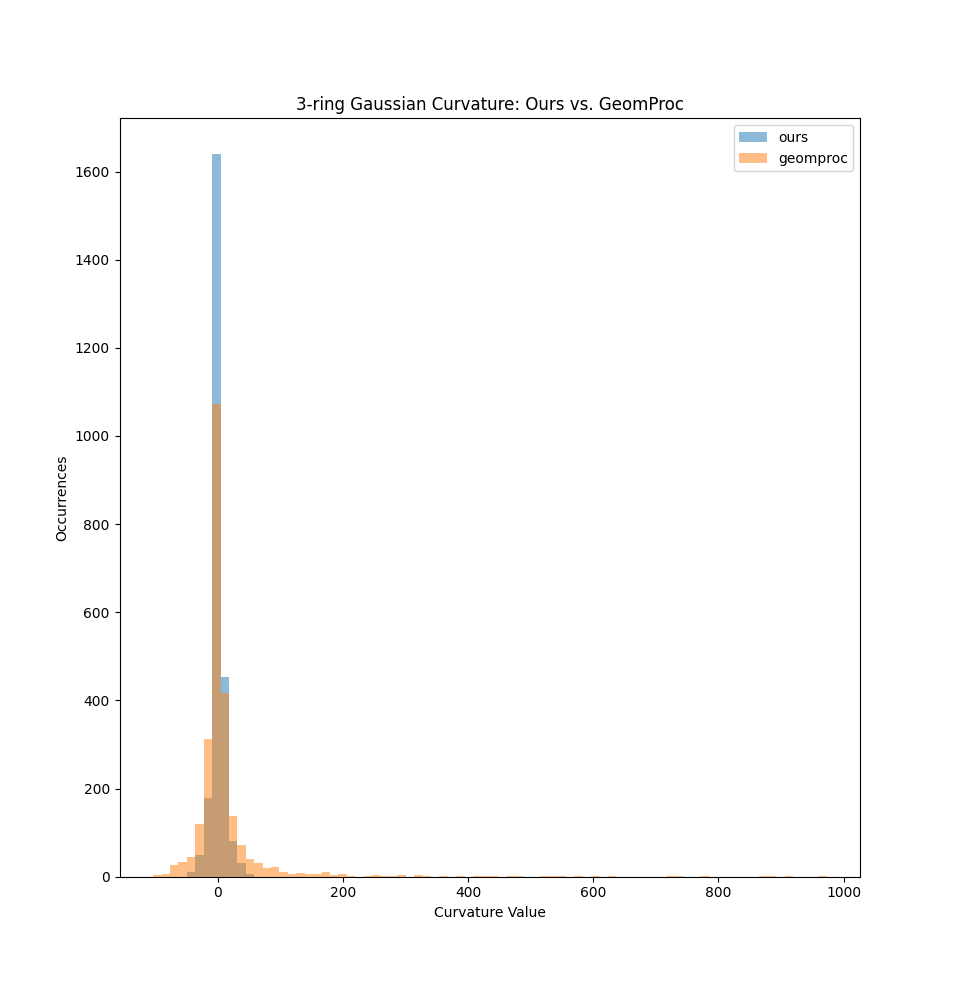
\includegraphics[width=1.5in]{gaussian_error_3.png}
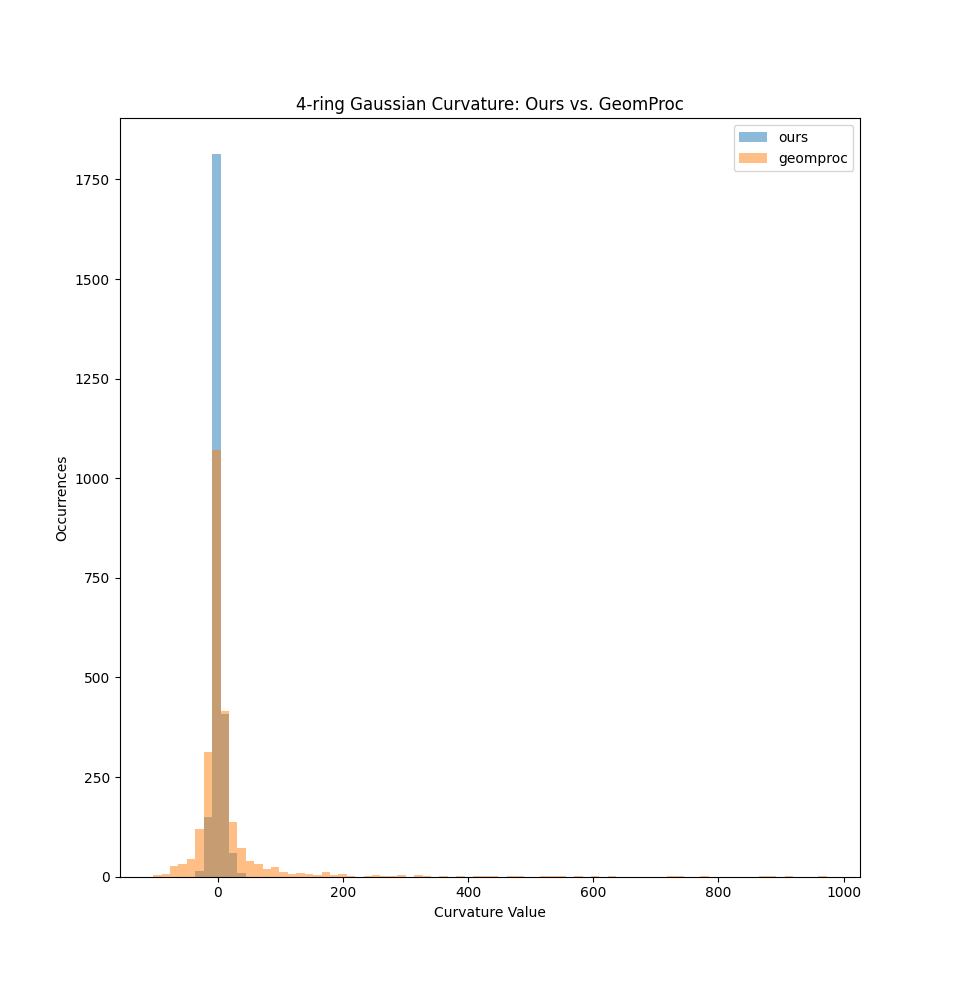
\includegraphics[width=1.5in]{gaussian_error_4.png}
}
\begin{center}
\b{\i{Visual Comparison: 1 to 4-ring from left to right}}
\end{center}
\smallbreak
\adjustbox{center}{
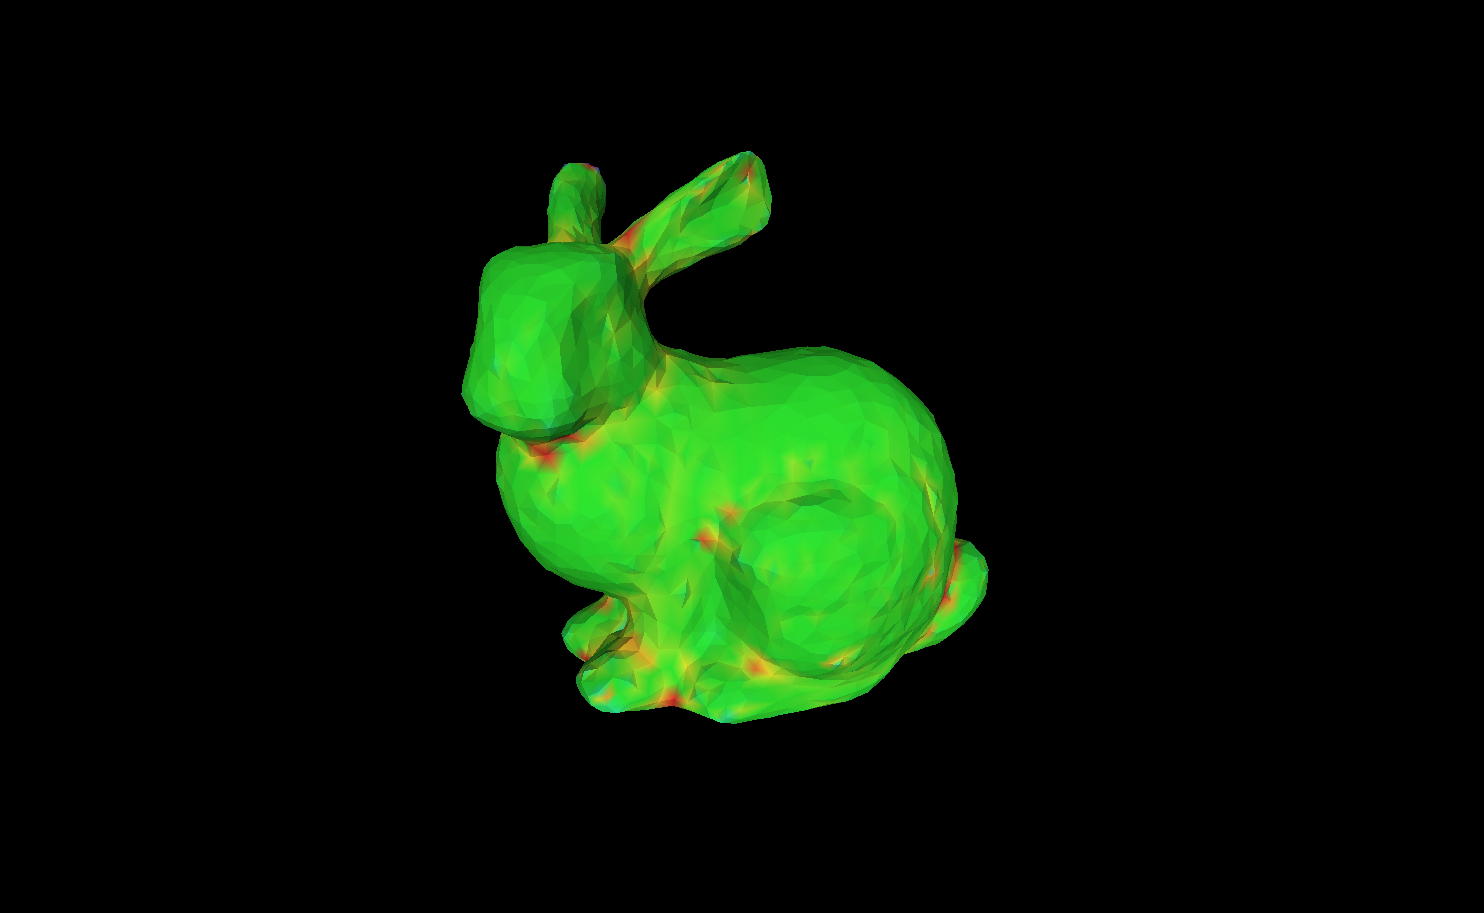
\includegraphics[width=1.5in]{gaussian_viz_00.png}
}
\adjustbox{center}{
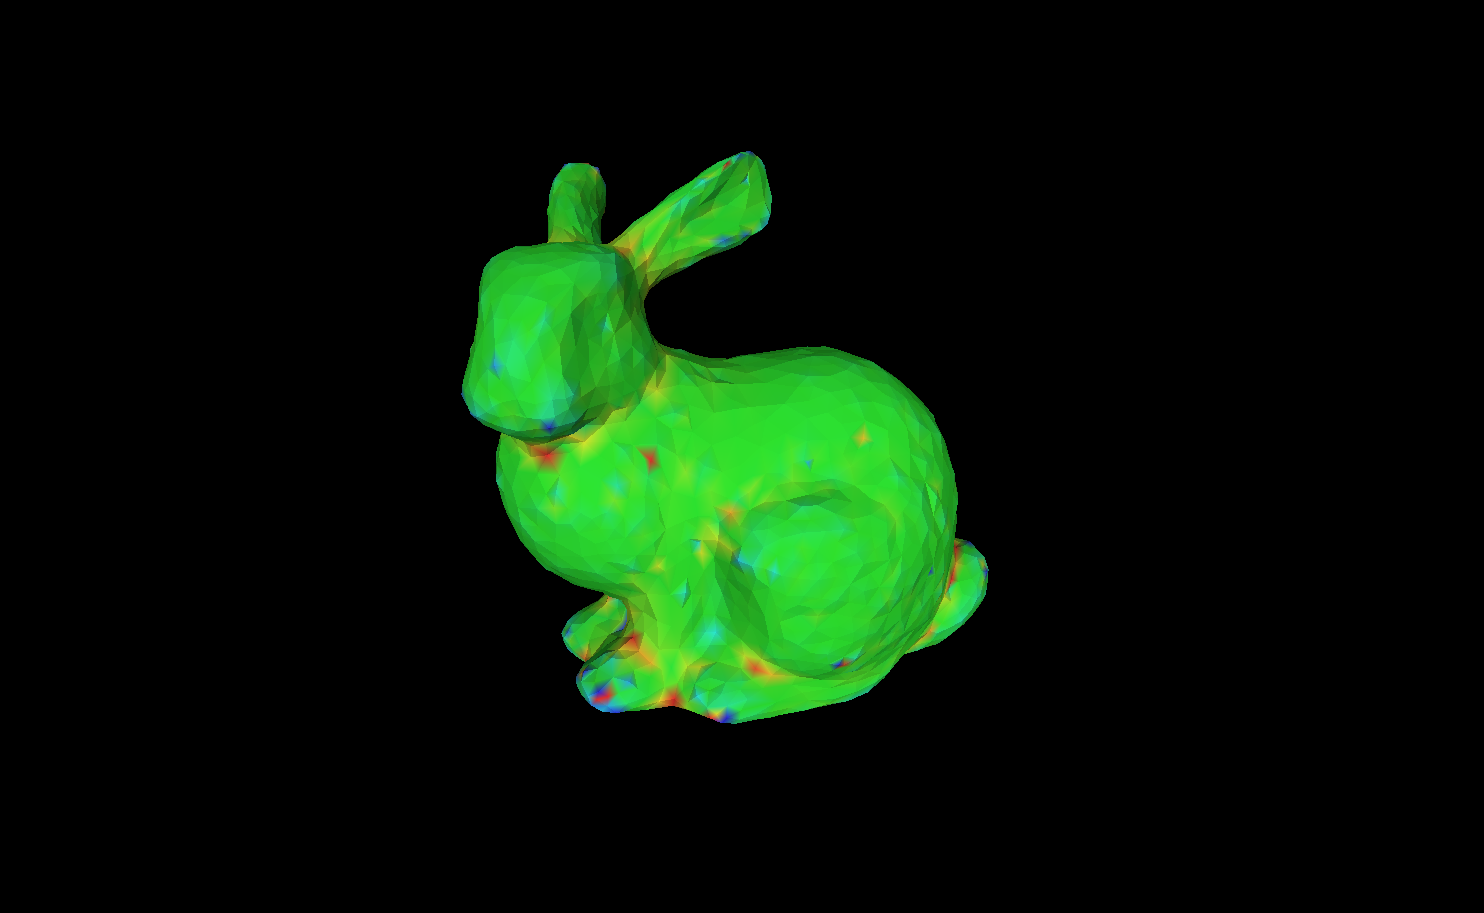
\includegraphics[width=1.5in]{gaussian_viz_01.png}
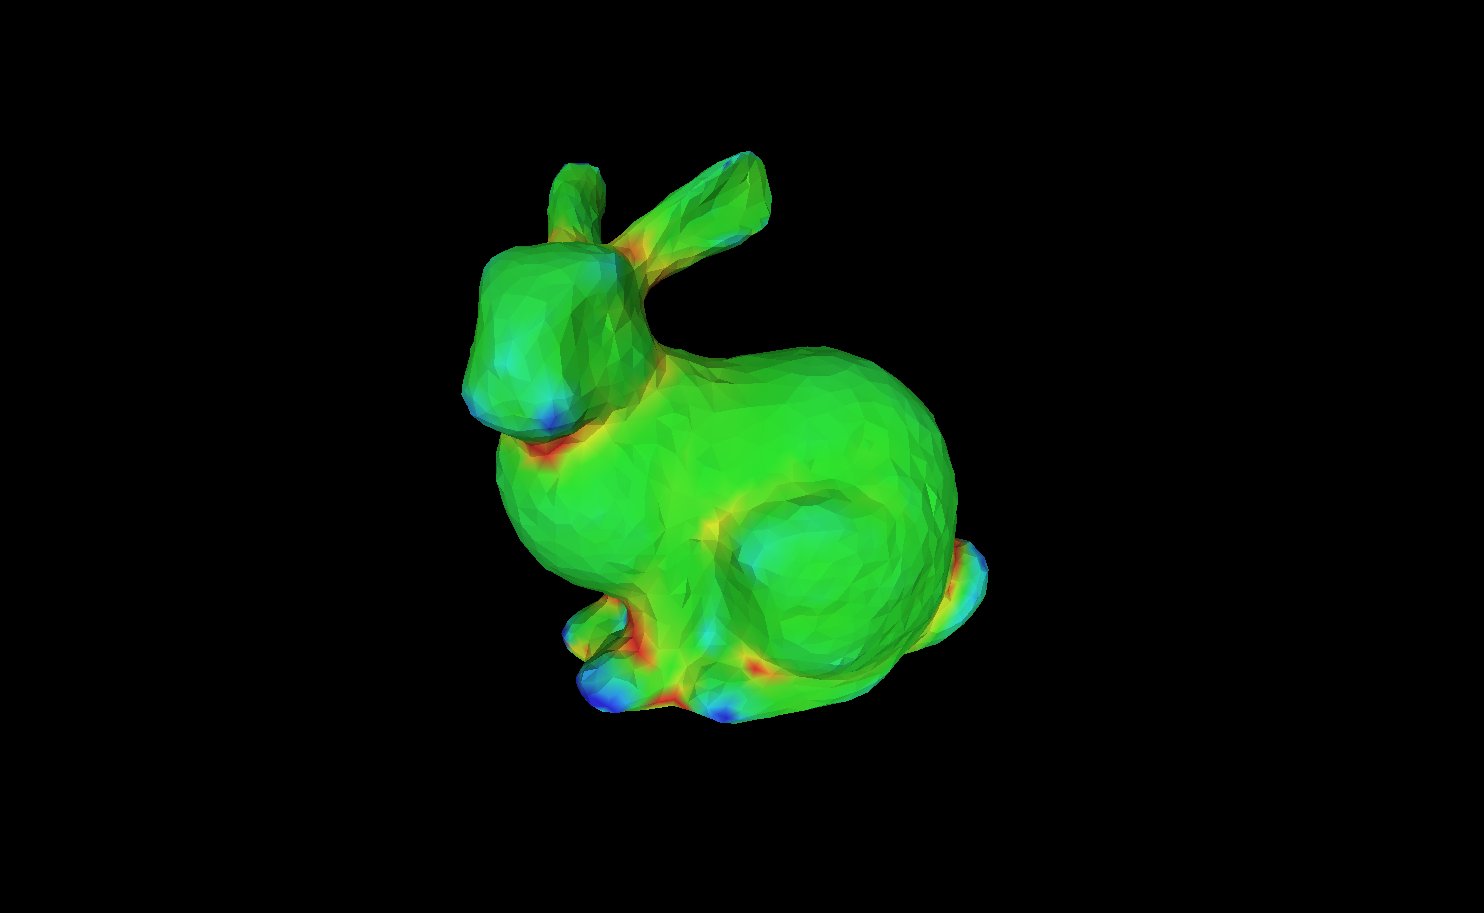
\includegraphics[width=1.5in]{gaussian_viz_02.png}
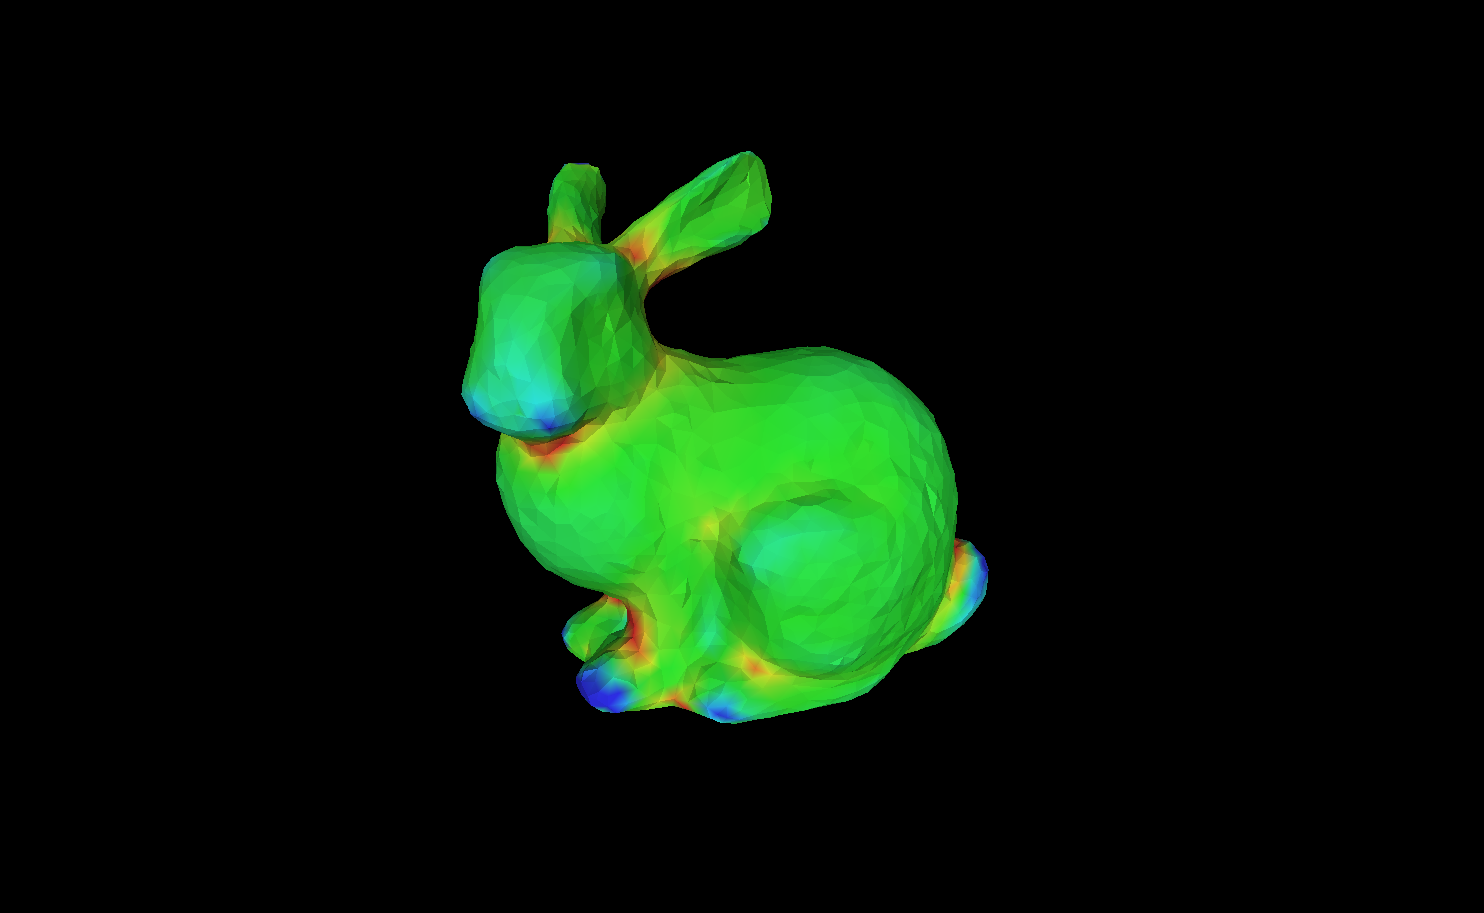
\includegraphics[width=1.5in]{gaussian_viz_03.png}
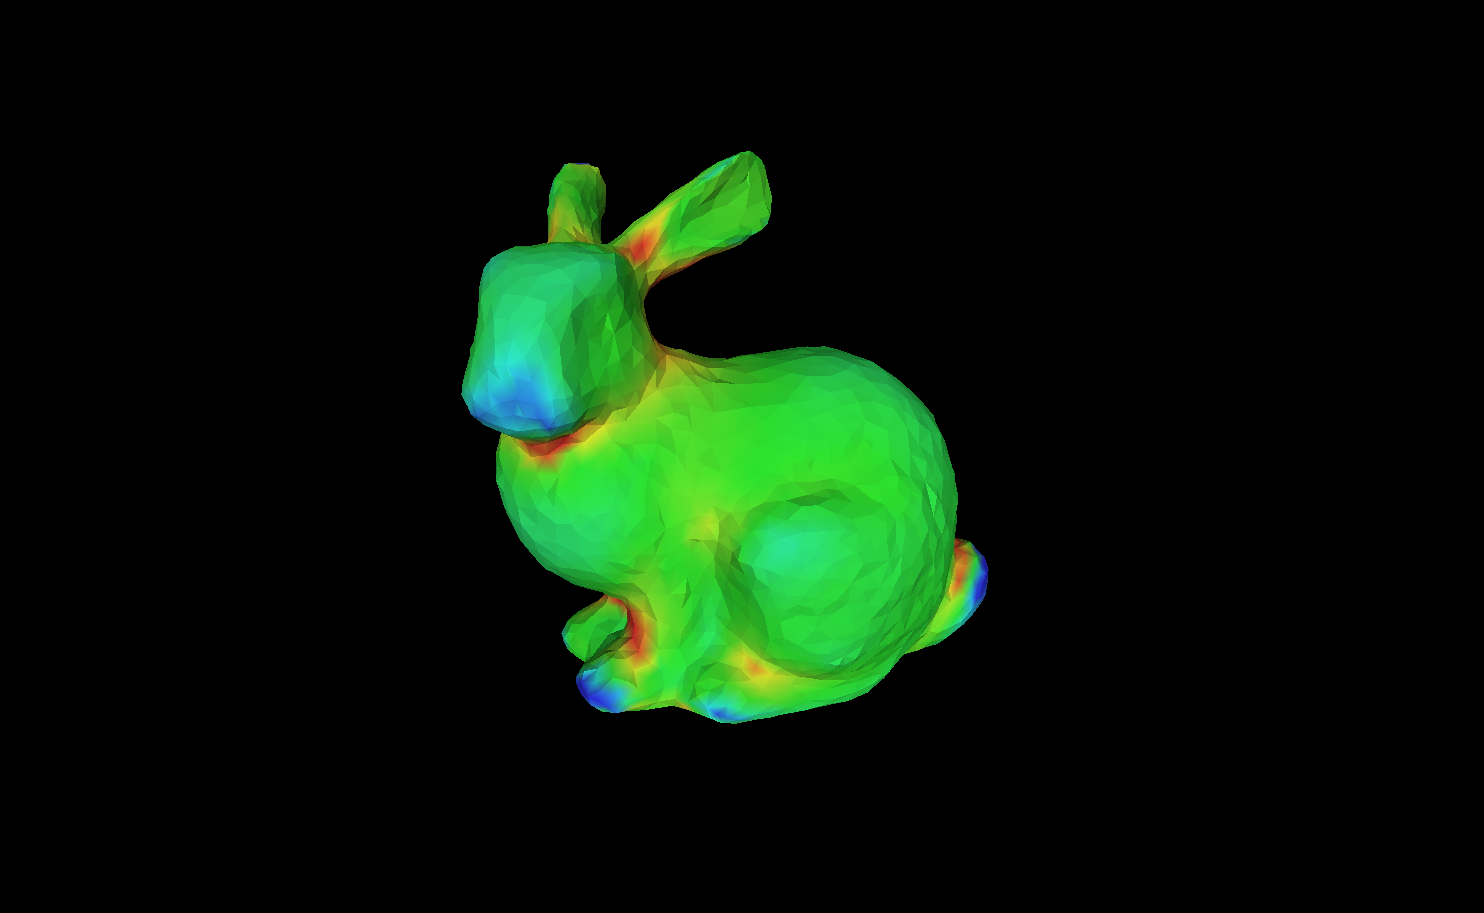
\includegraphics[width=1.5in]{gaussian_viz_04.png}
}

The polynomial surface gaussian curvature estimation outlined in the
specification resulted in a large MSE to the GeomProc baseline. From examing the
histogram results and visualizations, the GeomProc method has a long tail of positive curvature
values and is missing many of the negative curvature regions identified by the
polynomial method. This can be most notably seen in the 2-ring visualization,
the convex areas of the bunny are highlighted such as the nose, tail, and feet
where it is near zero on the GeomProc model. It seems there are almost no blue
regions on the baseline model. The 1-ring gaussian curvature model
seems to perform much worse than the GeomProc method as it contains more noise and doesn't
identify areas of high curvature that are highlighted in the control.
\pagebreak
\section{Results vs. Analytic}
\begin{center}
\b{\i{MSE to analaytic torus curvature}}
\smallbreak
\begin{tabular}{|c|c|c|c|c|c|}
    \hline
    1-ring Mean & 2-ring Mean & 1-ring Gaussian & 2-ring Gaussian & GeomProc
    Mean & GeomProc Gaussian\\
    \hline
    0.1186 &  0.3000 & 0.2475 & 0.8243 & 0.00004115 & 0.0005890\\
    \hline
\end{tabular}
\end{center}


\begin{center}
\b{\i{Visuals: Analytic mean \& gaussian vs. discrete (bottom same order as table)}}\\
\smallbreak
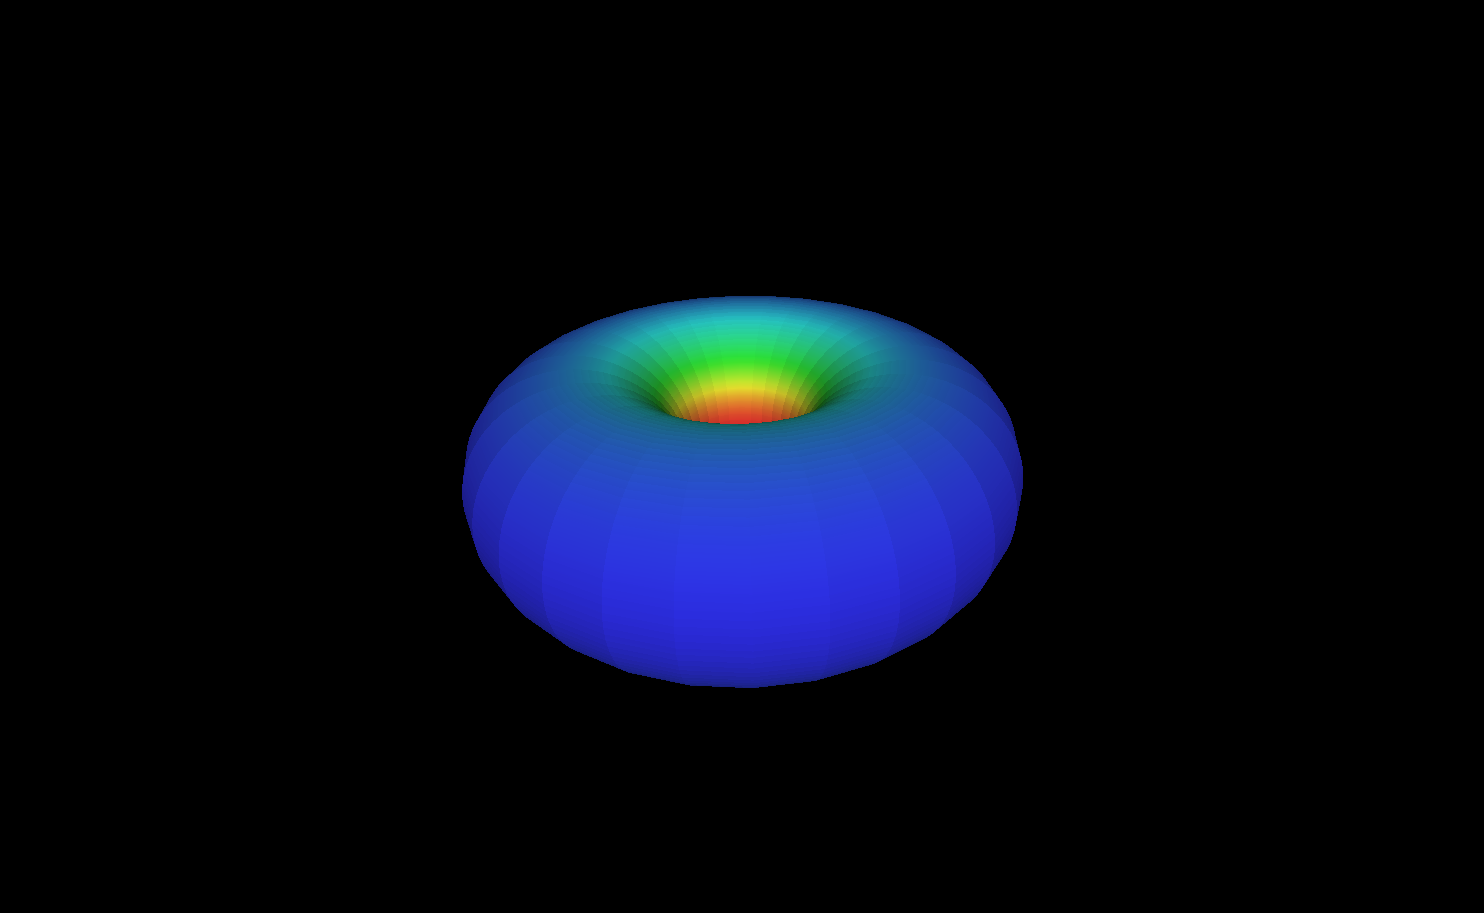
\includegraphics[width=1.0in]{torus_analytic_m00.png}
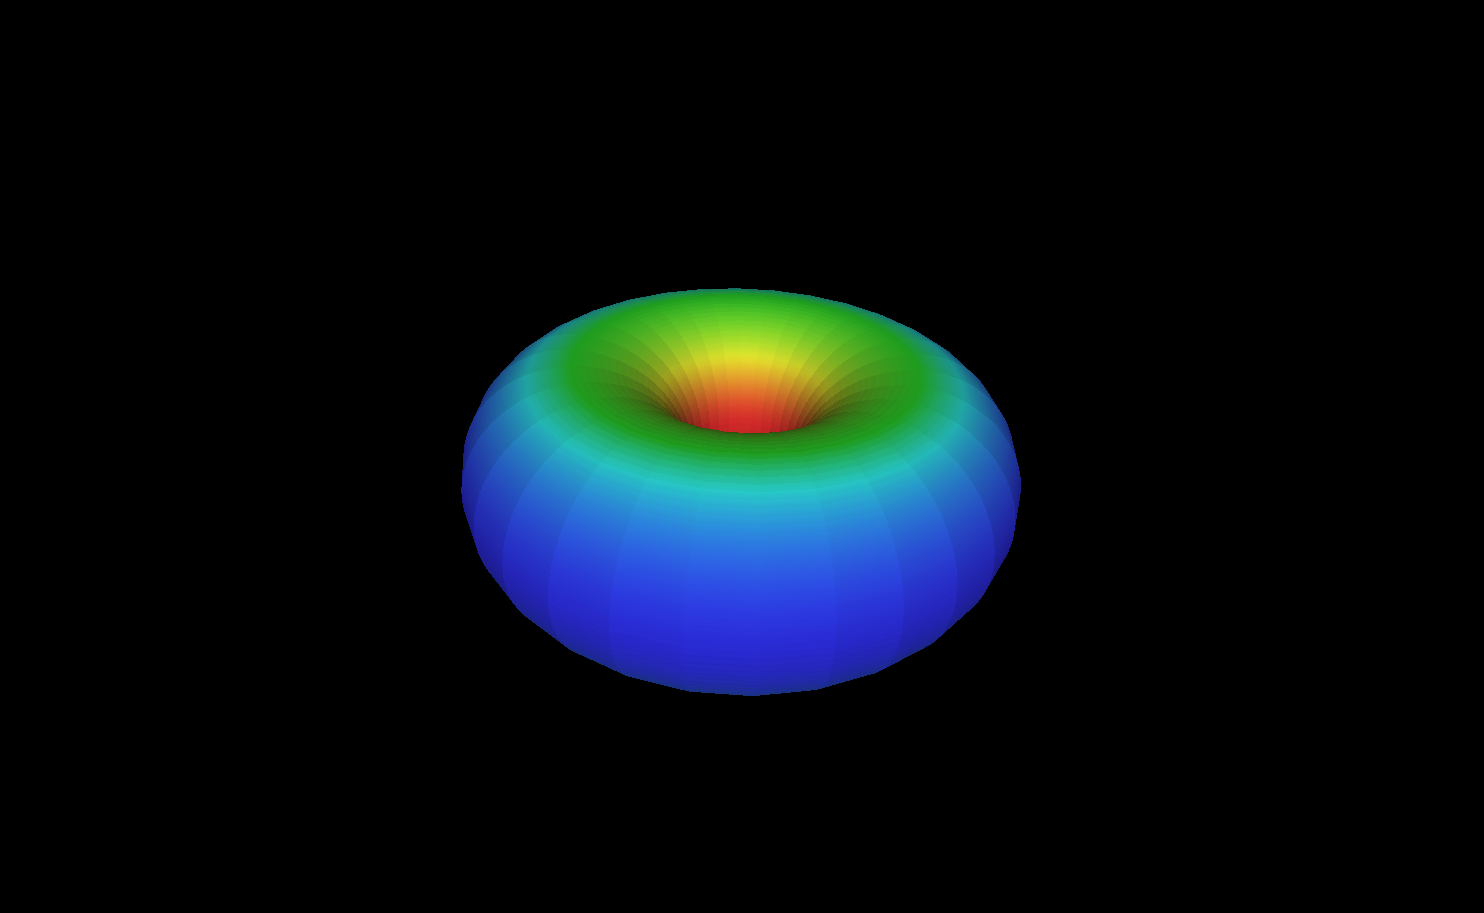
\includegraphics[width=1.0in]{torus_analytic.png}
\end{center}

\adjustbox{center}{
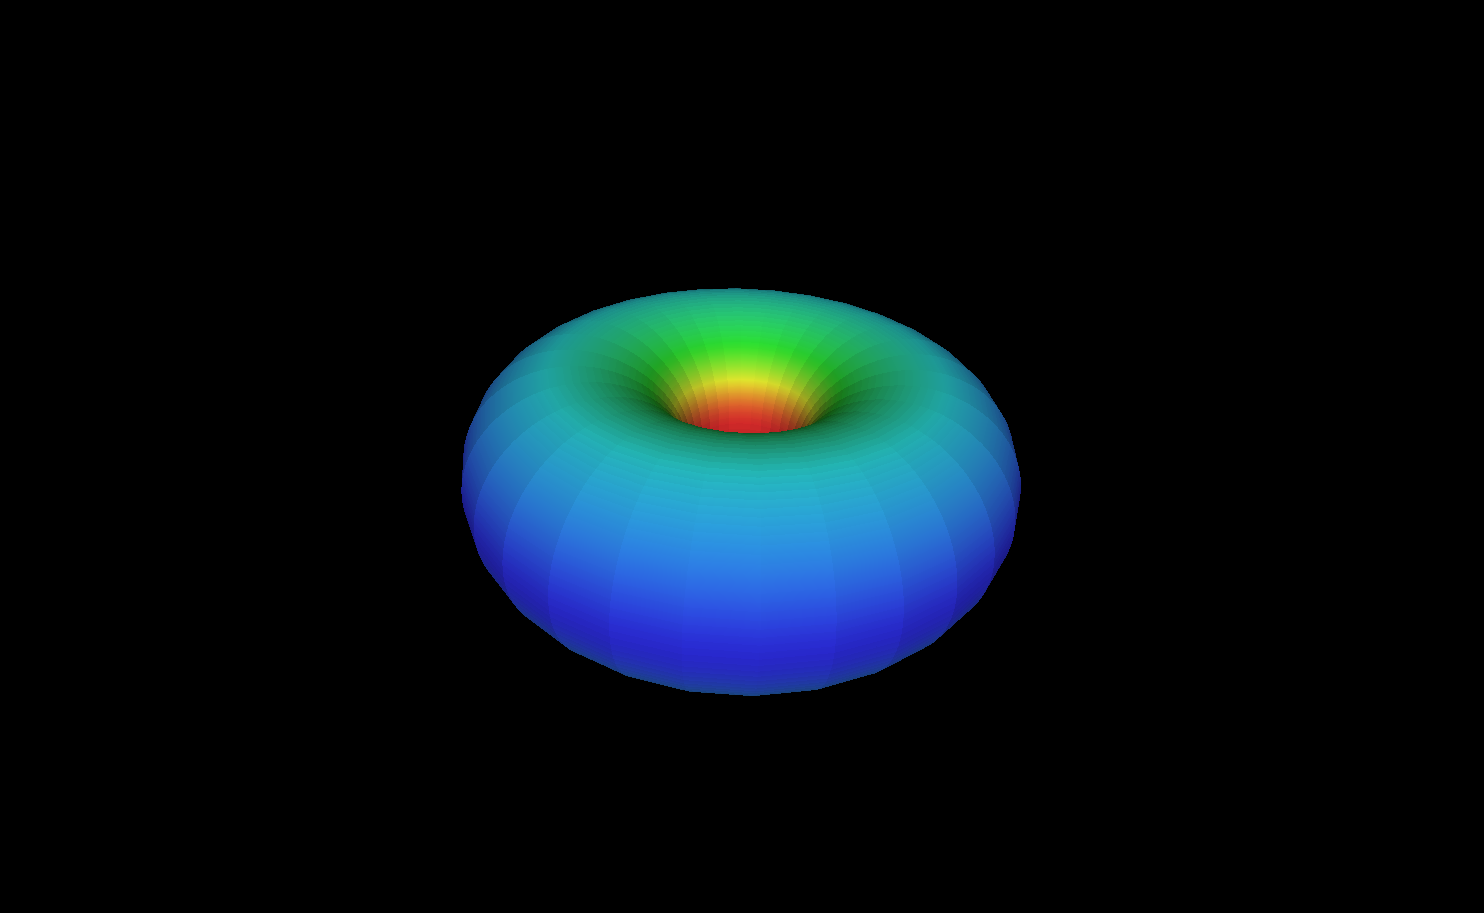
\includegraphics[width=1.0in]{torus_mean_01.png}
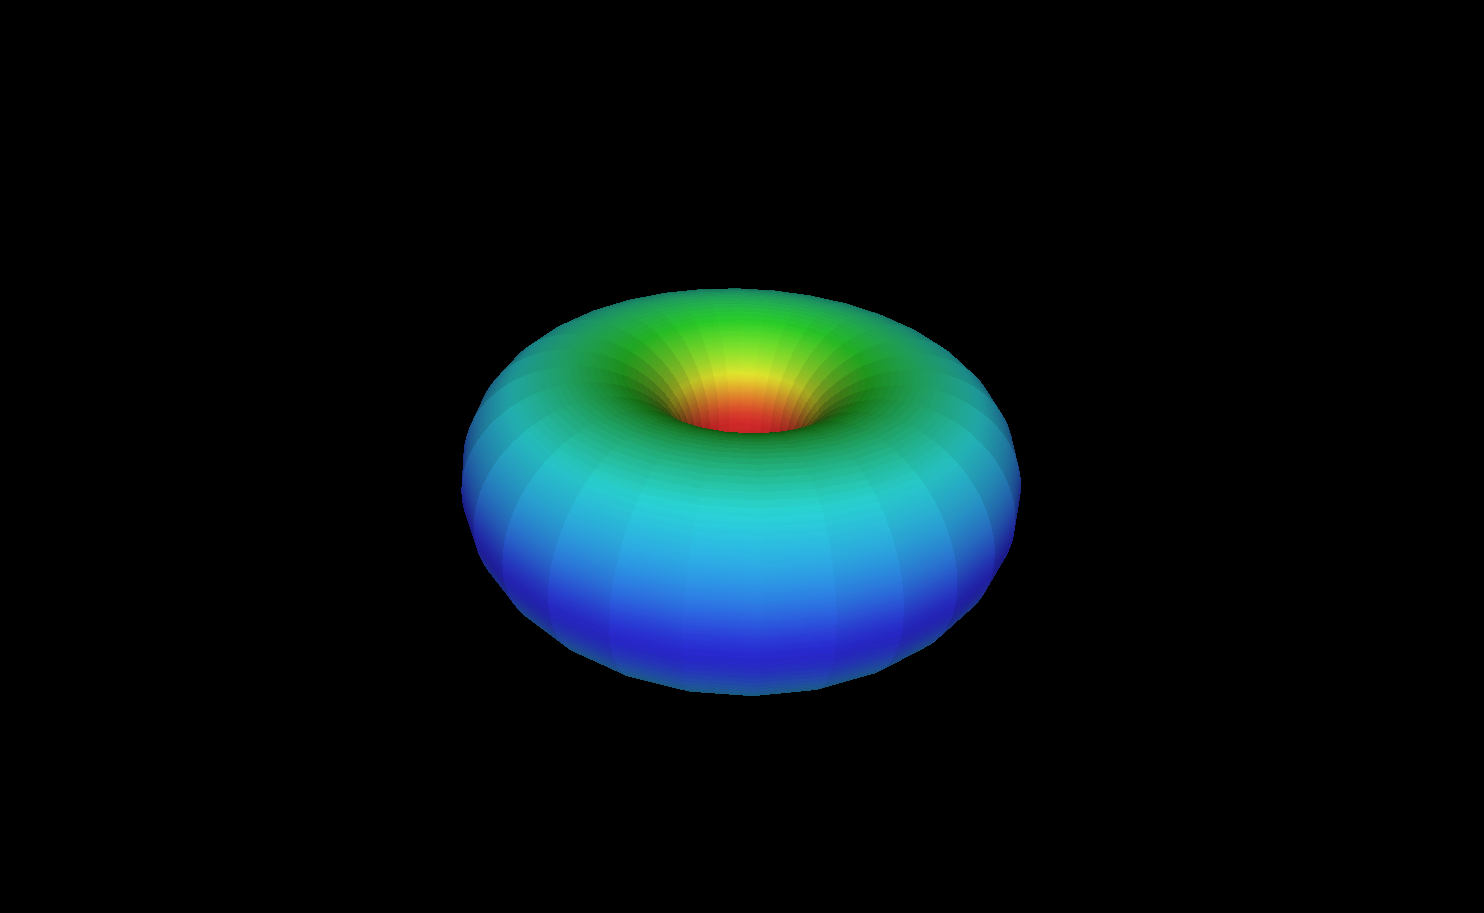
\includegraphics[width=1.0in]{torus_mean_02.png}
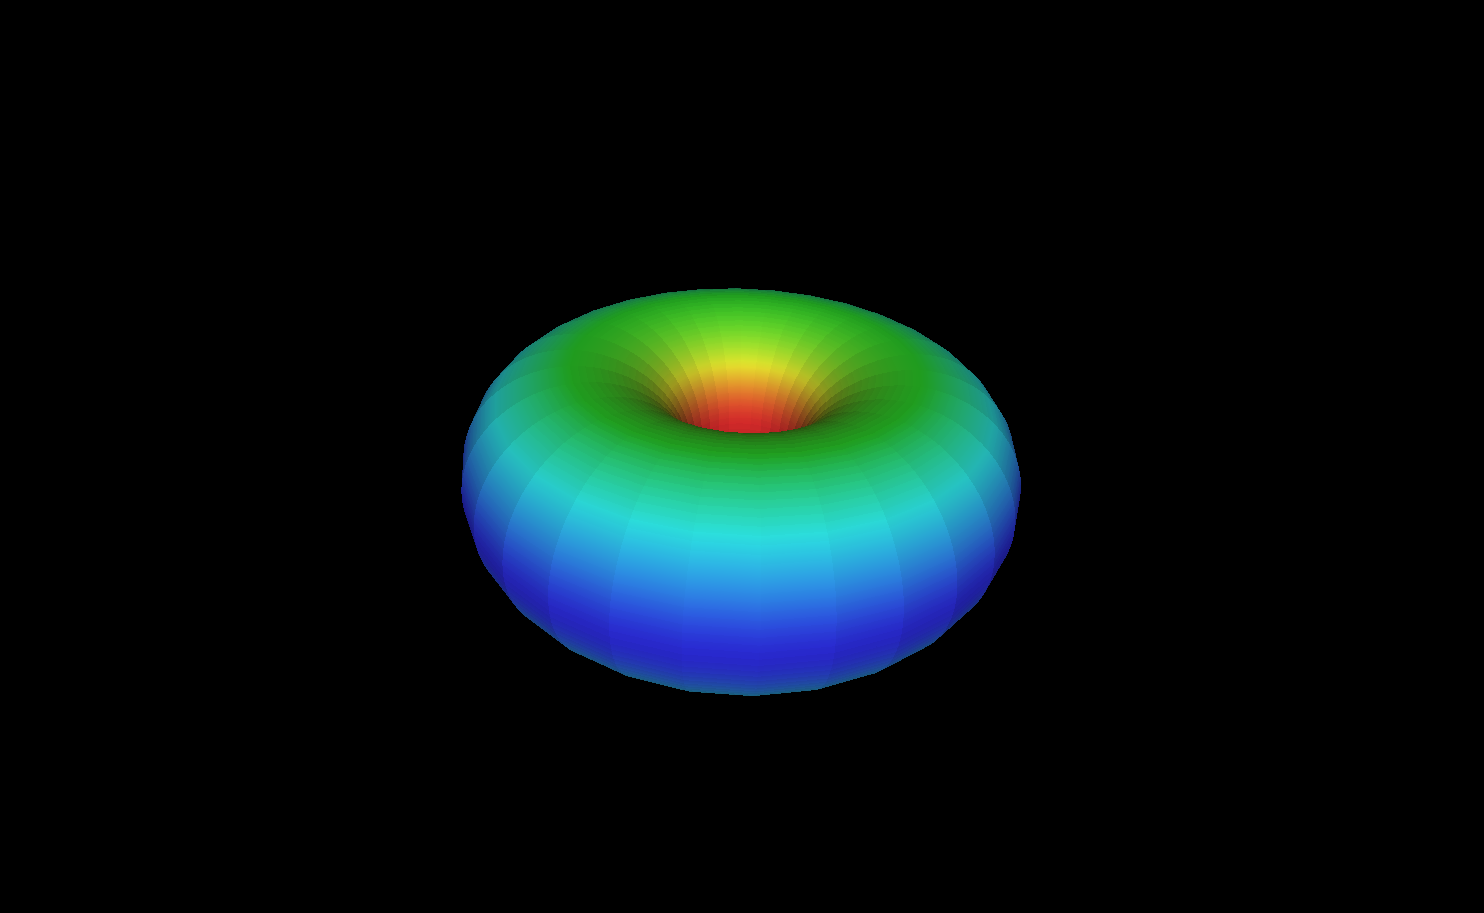
\includegraphics[width=1.0in]{torus_gaussian_01.png}
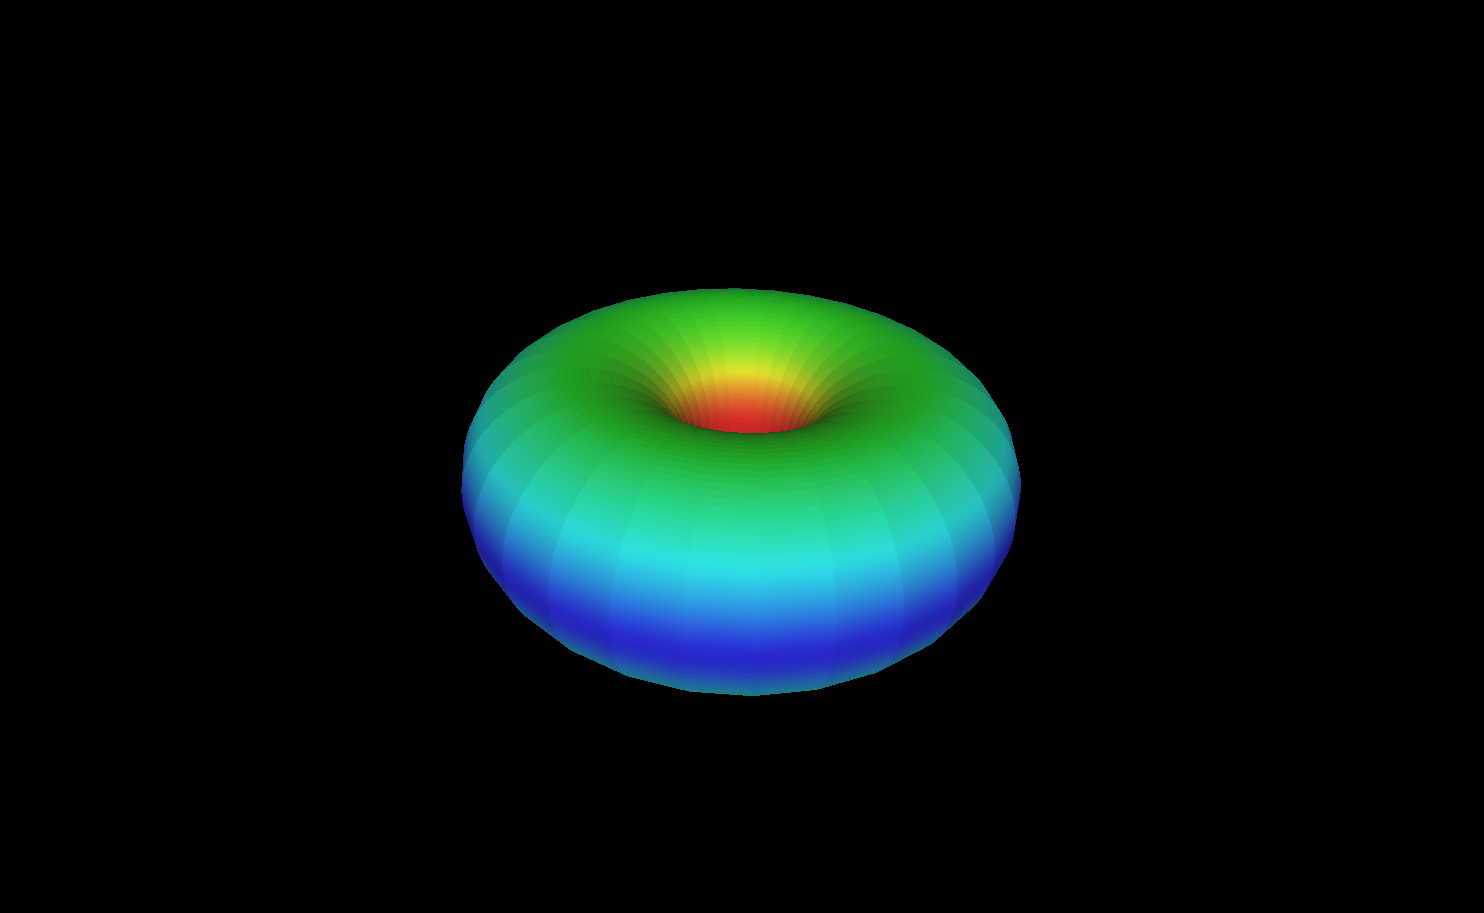
\includegraphics[width=1.0in]{torus_gaussian_02.png}
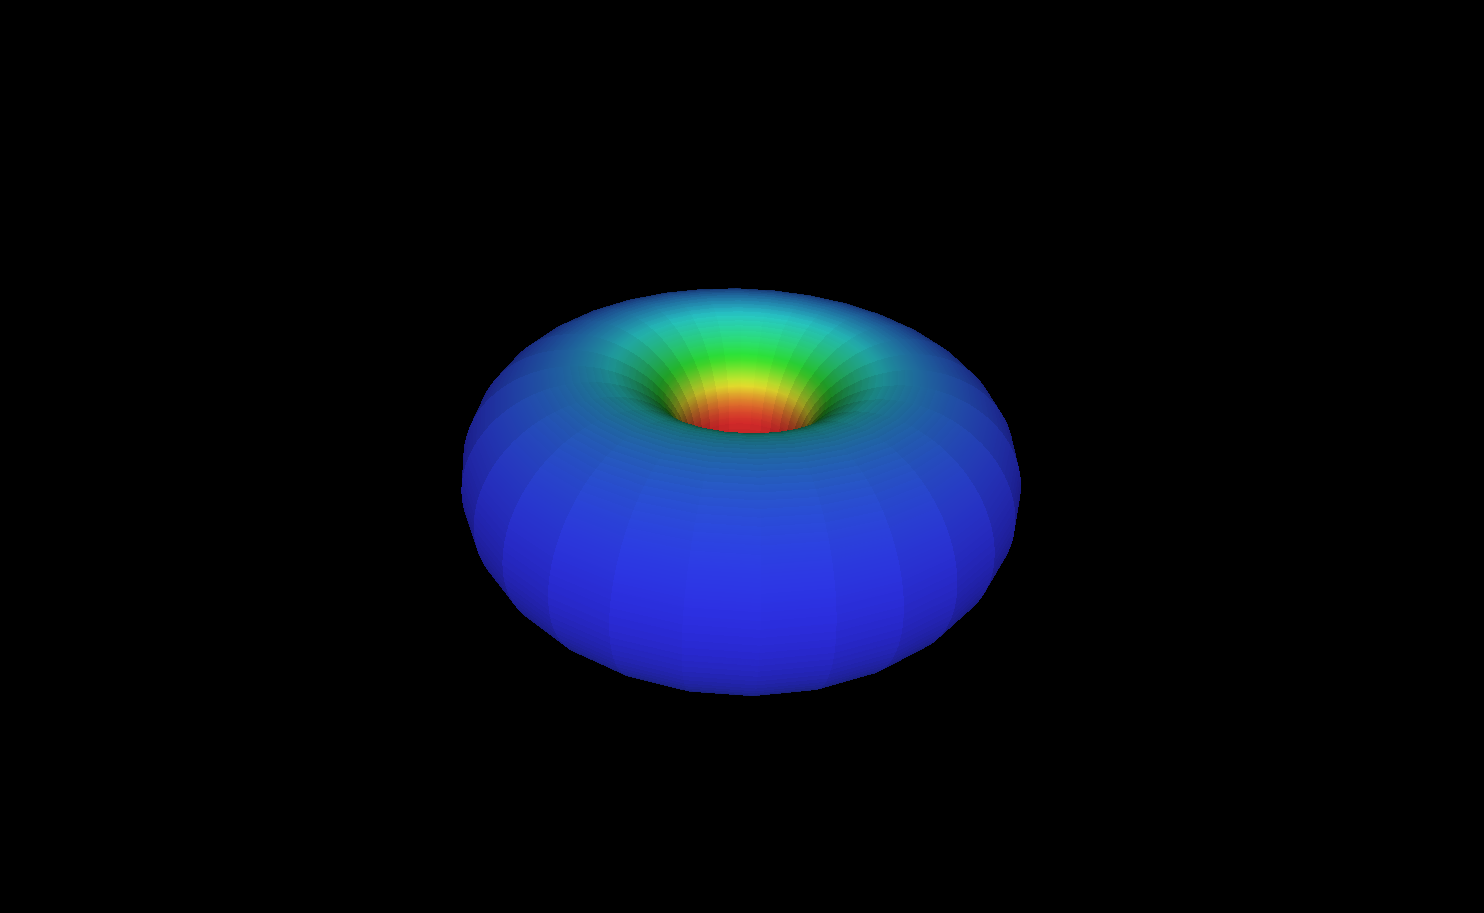
\includegraphics[width=1.0in]{torus_mean_00.png}
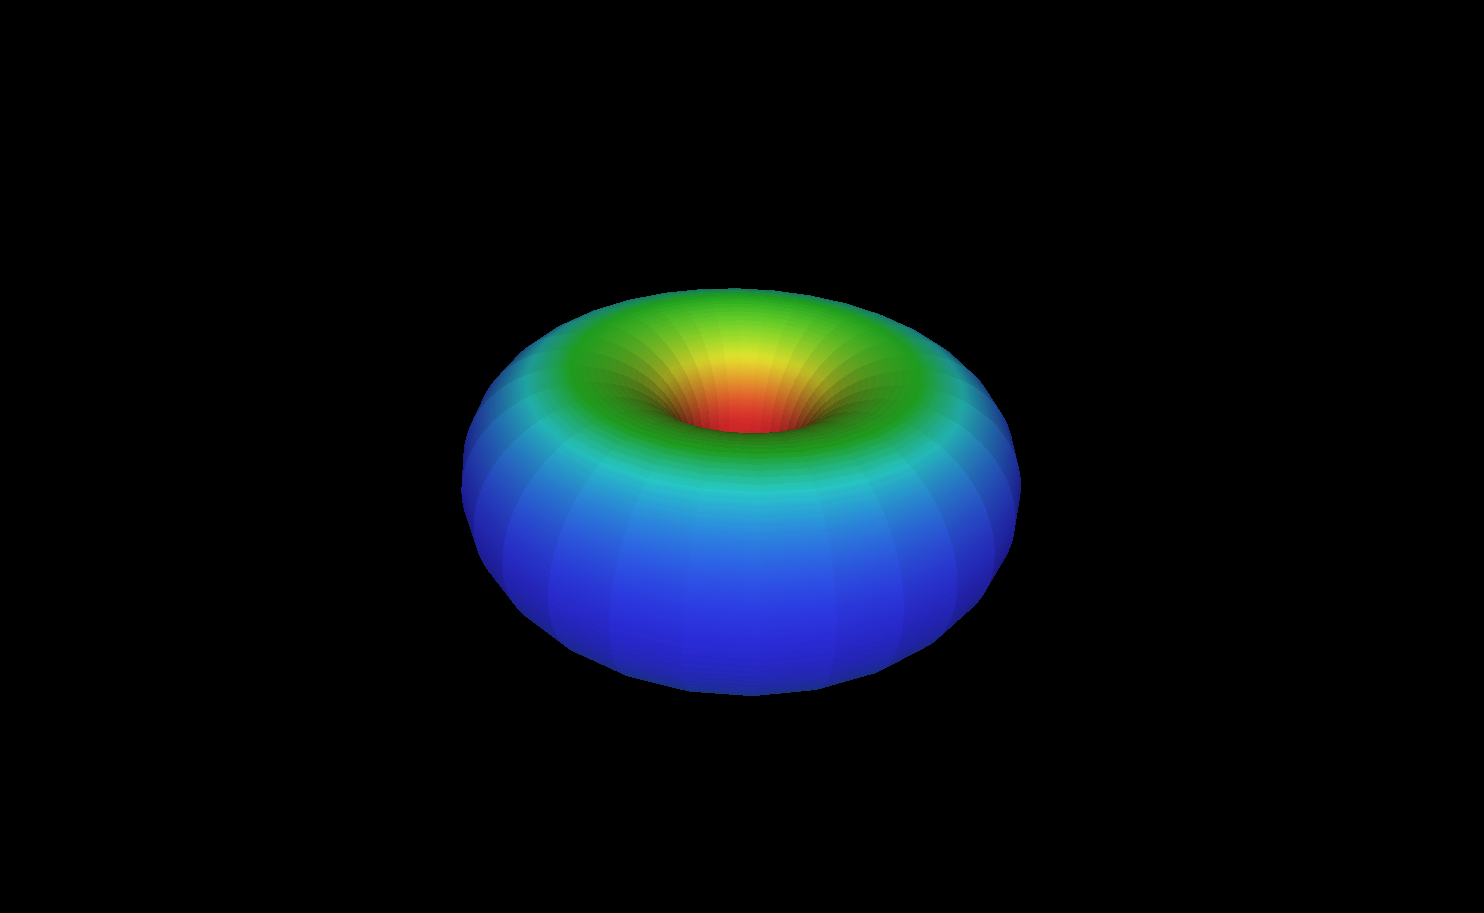
\includegraphics[width=1.0in]{torus_gaussian_00.png}
}
\bigbreak

\begin{center}
\b{\i{Curvature value distribution comparisons:}}\\
\smallbreak
\end{center}

\adjustbox{center}{
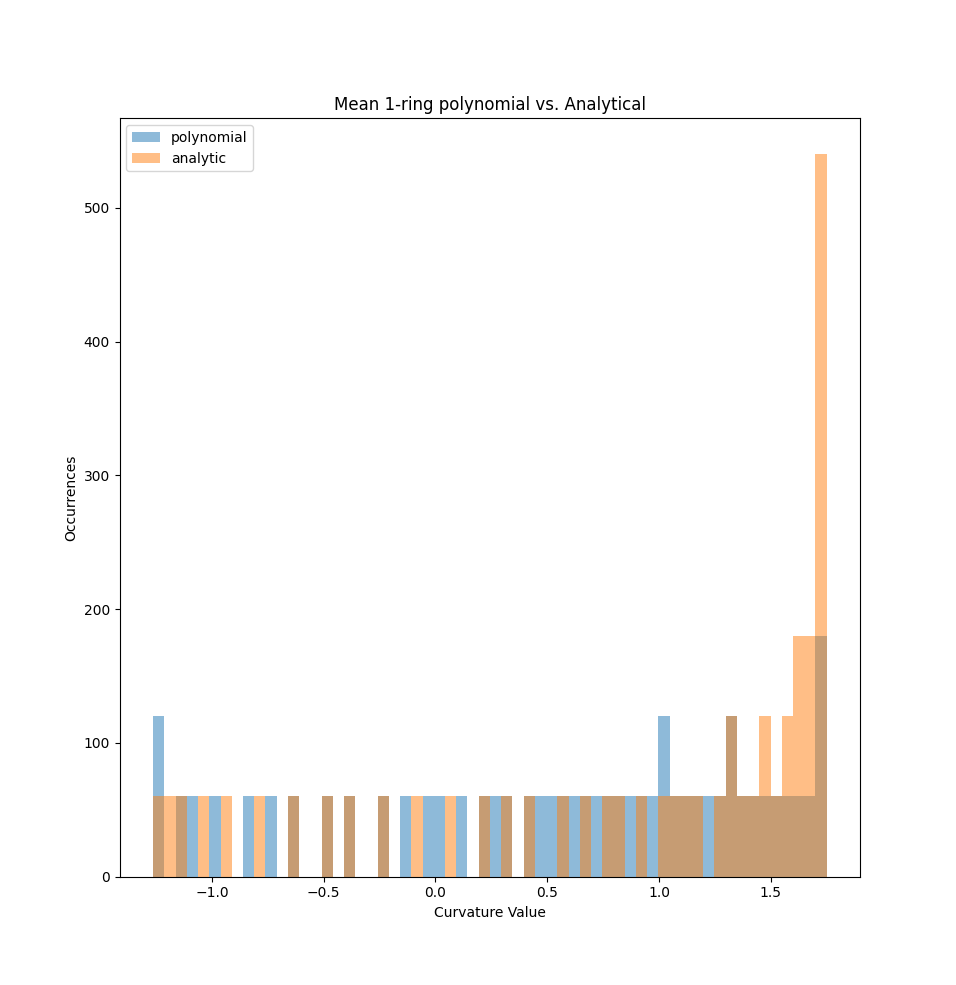
\includegraphics[width=1.2in]{anal_m_1.png}
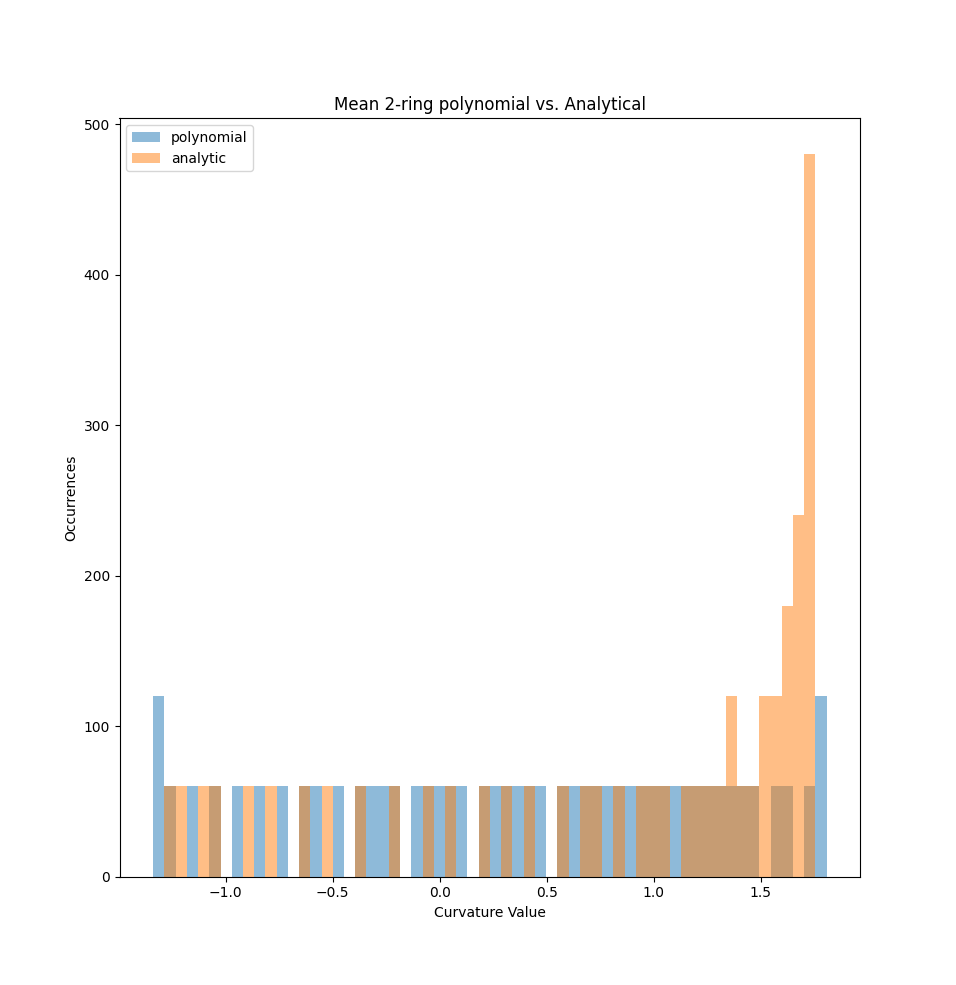
\includegraphics[width=1.2in]{anal_m_2.png}
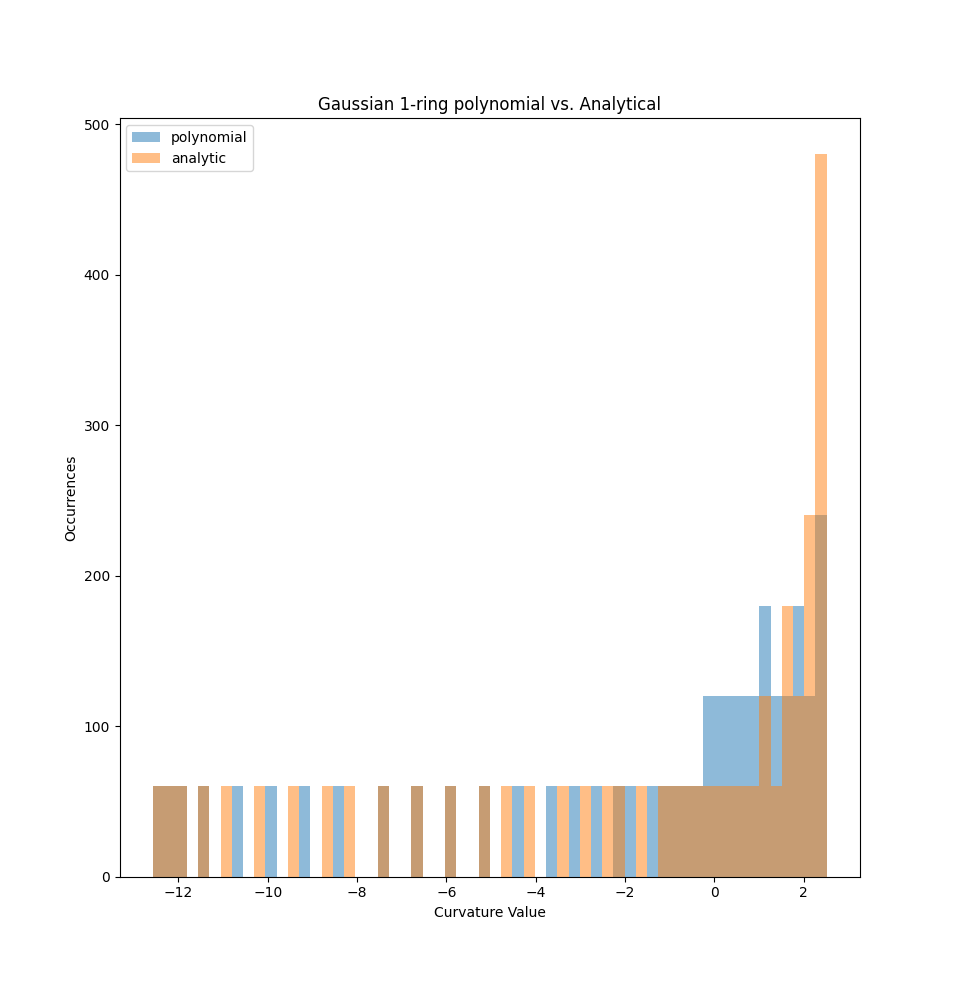
\includegraphics[width=1.2in]{anal_g_1.png}
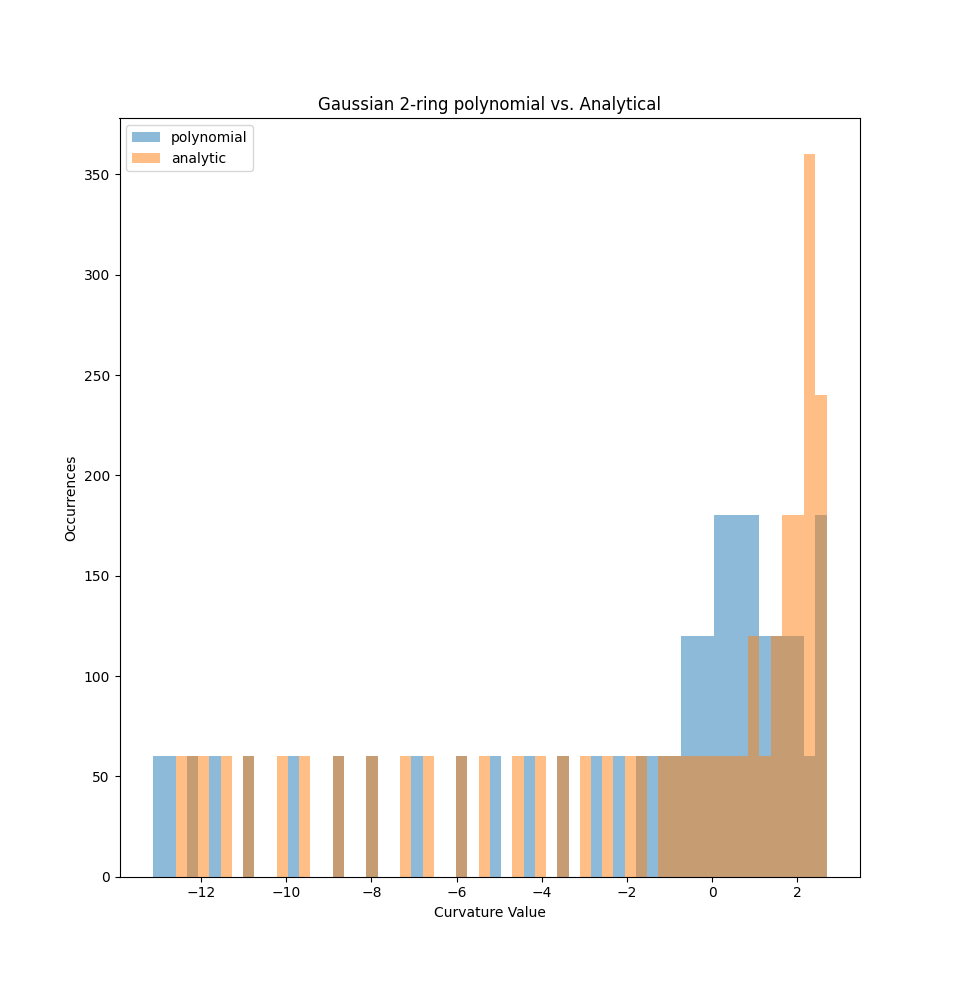
\includegraphics[width=1.2in]{anal_g_2.png}
}

\adjustbox{center}{
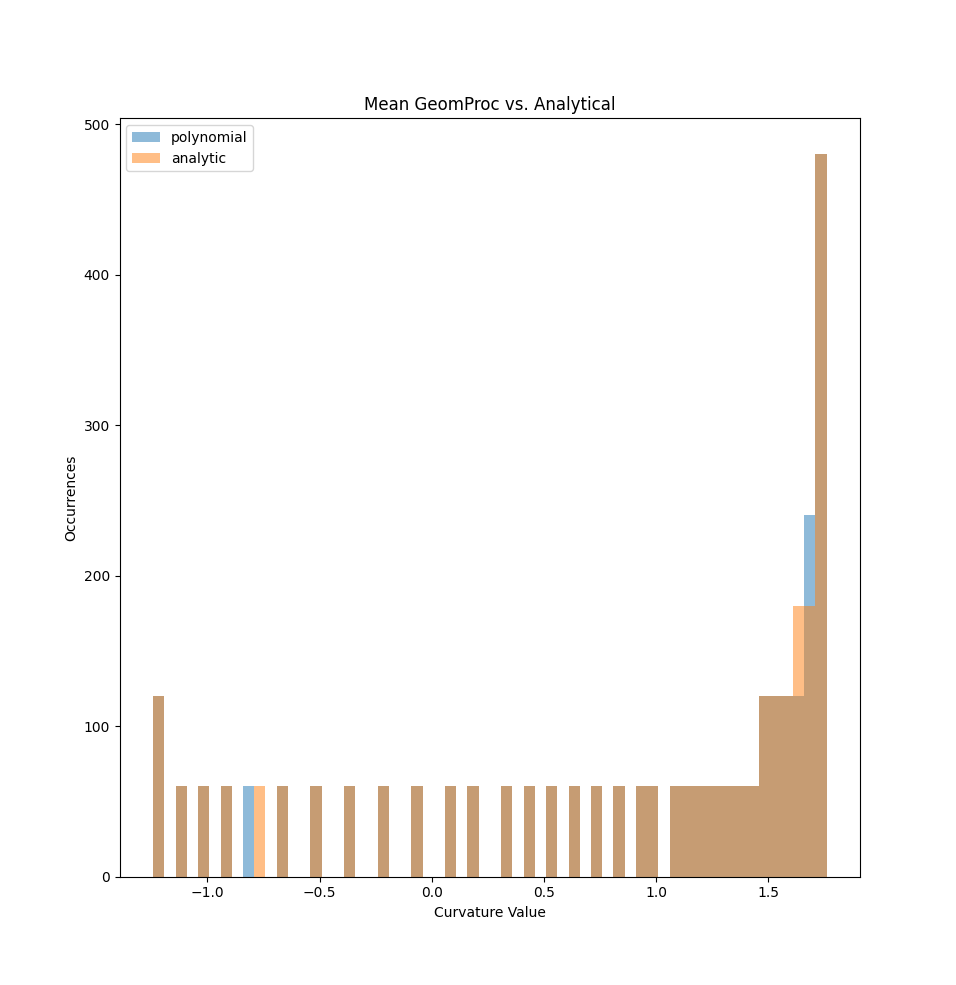
\includegraphics[width=1.2in]{anal_m_g.png}
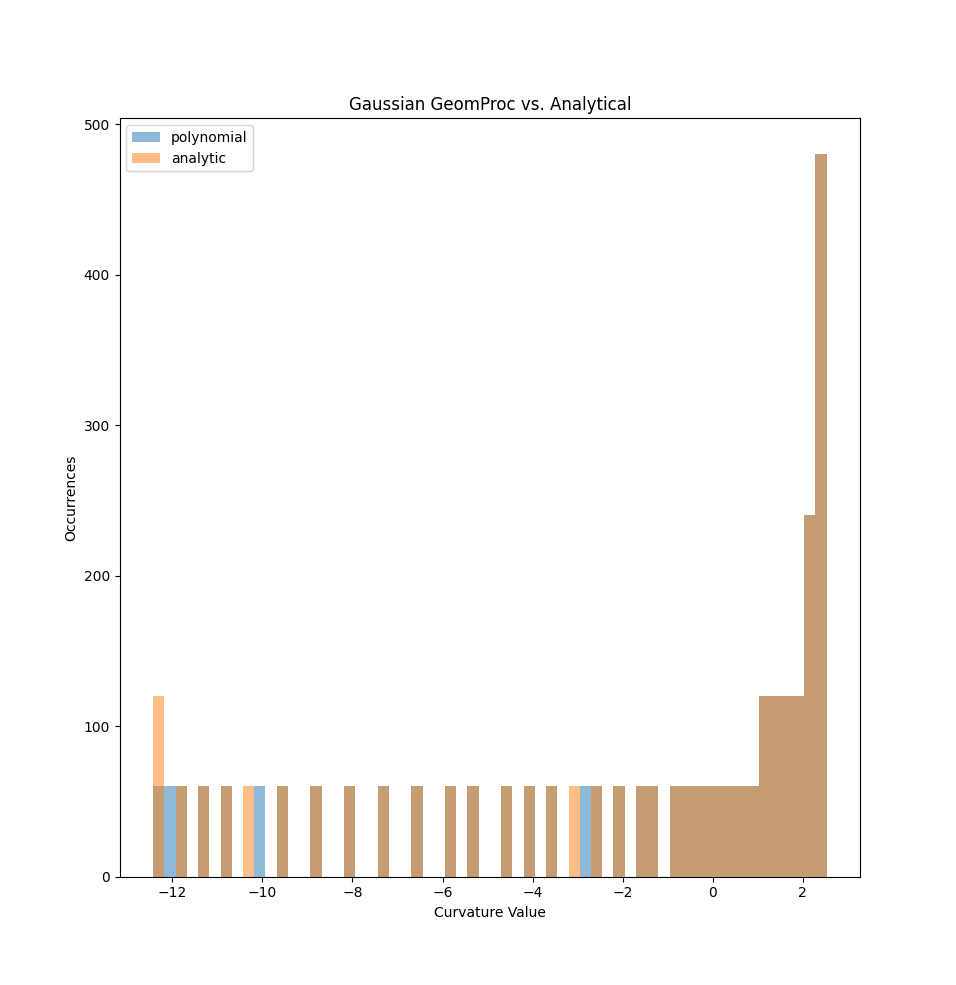
\includegraphics[width=1.2in]{anal_g_g.png}
}

In terms of replicating analytical curvature values with the least possible
error, the GeomProc Voronoi curvature estimation far exceeds the polynomial
surface fitting method. This can be seen by examining both the error values in
the table as well as how closely the GeomProc method fits the analytic
distribution of curvature. Visually, the Voronoi method also looks identical to
the analytic solution where the polynomial method has considerable differences
in color region and gradient. In conclusion, for the real-world models the
polynomial method seemed to produce more intuitive results, however, when trying
to minimize tiny error on an analytic surface, the GeomProc approach is the
better choice. 
\end{document}
